% ============================================================
%  第三卷 第十八章 非弹性碰撞（§142–§152 + 习题）
%  底本：高教社中文版第6版；OCR 错误已修正，脚注文本待从纸版补录
%  章标题行被 OCR 吞掉，章名"非弹性碰撞"按书前目录恢复（原书 p541 章首页已核实）。
%  主要 OCR 修正（行号为 full_merged.md 全局行号）：
%   1. 斜体 ι/\imath/\ell 下标误读 → l：S_l、f_l、P_l、δ_l、R_{kl}、g_l(k²) 等全章统一；
%   2. §142 截面下标恢复（按原书 p542）：σ_e（弹性）/σ_r（反应）/σ_t（总）；
%      行20789 (142.4) σ_r；行20795 σ_t=σ_e+σ_r；行20807 (142.7) 第二行 σ_r^{(l)}、
%      第三行 σ_t^{(l)}；行20813 (142.8)；行20827 (142.10) σ_t；行20837 (142.11) σ_t^{(l)}；
%   3. 行20771 (142.1) (ε−1)^{l+1} → (−1)^{l+1}（按原书 p541，同(123.9)）；
%   4. 行20766/20768 游离 ψ 记号删除；行20774 游离 S_l 归位于"只是 S_l 不再由…"；
%   5. 行20816 "当IS1|=1时"→当 |S_l|=1 时，行尾游离"2"删除；行20822 补句号；
%   6. 行20844–20856 割线绕行段游离记号归位：f(−k)=f^*(k)；行20847 成对公式不编号；
%   7. 行20874 (V/N)^{″3} → (V/N)^{1/3}；行20921 e^{−Nσ_t=1V} → e^{−Nσ_t z/V}；
%   8. 行20986 "Φ. . po,1958" → Ф. Л. Шапиро，1958（按原书 p547）；
%   9. 行21001/21005 (143.3)(143.4) 乱码竖线 → 4π|α|²(1−2k|α″|)、4π|α″|(1−2k|α″|)/k（p547）；
%  10. 行21008 游离 r^{-3} 归位于前句"衰减快于 r^{-3}"；行21010 游离 r^{-2} 删除；
%  11. 行21024 游离 Z_1e/Z_2e 归位为"其中 Z_1e 和 Z_2e 是相碰粒子的电荷"；
%      行21036 exp(ħ−2πZ₁Z₂e²/ħv) → exp(−2πZ₁Z₂e²/ħv)；
%  12. §144 下标乱码：行21095/21182 f̂_ℏ→f̂_fi、f_ℏ→f_fi；行21129 (144.11)
%      S_{i·p·d}→S_{i^*f^*}；行21135 (144.12)；行21145/21165 dσ_{i·f*}→dσ_{i^*f^*}、
%      do_{i·}→do_{i^*}；行21171 σ̄_i→σ̄_{fi}；行21150 f_{fi}=f_{if}；行21044 行尾"8"删除；
%  13. §145 全节 OCR 的 T→Γ（(145.1)–(145.17) 及正文，按原书 p552–555）；
%      行21215 (145.2) k_a→k_c（按原书 p553）；行21283 e^{2iδℓ⁰)}→e^{2iδ^{(0)}}；
%      行21348 "E=0 值"→E_0 值、ε。→ε_0、Γ。→Γ_e；
%  14. 行21390–21417 平均模型截面记号 σ_e^−/σ_a^* → σ̄_e^光/σ̄_r^光（按原书 p557–558）；
%  15. §146 行21435/21449/21455/21483 "常数×"乱码（ŋŋ/♯♯χχ 等）→ \text{常数}；
%      行21477 (p_⊥²+p_∥²)/m 归位；行21480 p_#→p_∥；行21430 P。/P→p_0/p；
%  16. §147 阈值下标乱码 \bowtie/\mathrm{fsf}/\astrosun/pq/\mu\nu/\check\imath 等 → 阈
%      （E_阈、k_阈、f_阈、σ_阈，按原书 p562–565）；行21504 "A. . Ba3b"→А. И. Базь；
%      行21537 (147.7) S_{ss}→S_阈；行21530 "方括号内"→"括号内"（(147.6) 为圆括号）；
%      行21588 (147.11) 常数乱码→常数；行21658 括号不配 (…]→[...]；
%  17. §148 行21705 脚注圈码①按原书 p567 系于公式 (148.3) 编号后，排于公式后正文之首；
%      行21708 补句号；行21787 (148.13) "H·J"→"时"；行21829 "sinϑ do"→"cosϑ do"
%      （按 dε=E·2sinϑcosϑdϑ 校核）；行21845 (148.18) 矩阵元模量归位；
%      行21853 (148.19) 分子乱码→常数；行21863 (148.20) 第二行 (2e²/mv²)²do/ϑ⁴；
%      行21920 题1 (v^{-2}<<ϑ<<1)→(v_0/v)²≪ϑ≪1（按§148正文条件，原书 p572 印作 v^{-2} 系误）；
%      行21930 "物物坐标"→"抛物坐标"；行21951 题2 结果 n′→n^7（按原书 p572，并对
%      n₁−n₂ 求和 Σ(n₁−n₂)²=n(n²−1)/3 校核）；行21982 题3 积分上限 ε₂→ε_max；
%      行22007 题4 (1−e^{−2πκ})→(1−e^{−2π/κ})（同页第二处同因子即作 −2π/κ）；
%      行21991/22001 题4 中 \mathbf{\varepsilon}→ξ；
%      行21918 "习题①"圈码①属习题标题（脚注：所有题都采用原子单位），暂置于(148.26)之后；
%  18. §149 行22182 "σ_1"→ε_1；行22197 √(½ε)→√(e/2)（按推导校核：e 为自然对数底，
%      结果 ln(v²/0.94)）；行22121 (149.8) 补矩阵元右竖线；
%  19. §150 行22263 (150.7) 编号尾部句点删除；行22268 行尾扫描噪声"AU"删除；
%  20. §151 行22353 (151.5) f_a^{*}→f_a^{+}；行22377 题1 e^{−iφ·R_a}→e^{−iq·R_a}；
%      行22385 题2(1)式 q·ν/2→q·r/2；行22411 题2(2)式 (f^{*}+f^{-})²→(f^{+}−f^{-})²；
%  21. §152 行22539 (152.8) "S,"→S(ρ,…)；行22536 "类似于"后游离 \textcircled{1} 删除；
%      行22495/22563 (152.2)(152.12) 核波函数 φ_i→Φ_i（全书统一）；
%      行22609 题1 ψ_a→ψ_d；行22638 "氚核"→"氘核"；
%      行22644 "Φepr"→Е. Я. Фейнберг、"Axep；A. Γ.1955"→А. И. Ахиезер; А. Г. Ситенко，1955
%      （按原书 p588）；行22652 \mathbb{D}→①；行22675–22681 俘获/衍射截面下标乱码
%      →σ_俘获、σ_衍射（俘获下标按原书 p588）；行22720 "被俘"→"被俘获"。
%  遗留问题：
%   - 行21985 §148 题4 I 的指数按原书 p573 照排为 exp(−iq·r−iκr−λr)（按抛物坐标还原疑应为
%     −iκ·r）；抛物坐标式中 F(−i/κ,1,−iκξ) 与笛卡儿式 F(i/κ,1,i(κr+κ·r)) 的参数差异照原书保留；
%   - 行21364 "b+Y 粒子系统"照原书 p556 排印保留（疑为原书排版残留）；
%   - 行22032 (149.1) 后圈码①原书在句号后（"……而言的.①."），本稿置于句号前；
%   - §152 题2 编号 (1)(2)(3) 与题1 编号 (1)(2)(3) 各自独立（按原书 p588–590）。
%  脚注转录（脚注代理）：
%   - 全章圈码 54 处：53 处转录为 \footnote{}（按 pages300 页面实况逐一核对），
%     1 处为正文交叉引用（§152 题1 "见534页注①"，指 ch17b p534 脚注①），
%     按 ch16 先例改排 {\symbol{"2460}} 保留字面圈码，非脚注。
%     页码分布：p556×2、p557×1、p558×2、p559×1、p560×2、p561×1、p562×1、p563×1、
%     p564×1、p565×3、p566×1、p567×1、p568×1、p569×1、p570×2、p571×1、p572×3、
%     p573×1、p574×1、p575×1、p576×1、p577×3、p578×2、p579×1、p580×1、p582×1、
%     p583×3、p584×0（p585×1）、p586×1、p587×1、p588×1、p589×1、p590×1、p591×1、
%     p593×1、p594×1、p598×3、p599×1、p601×1（p596 无脚注页）。
%     （对照表缺行20870 之外诸行页码者，均已按页面实况核实归属。）
%   - 公式类脚注：p578 脚注①含极限表式 ψ(x)≈ln x−1/2x（equation*）；p582 脚注①
%     含 |⟨n|d_x|0⟩|² 式；p583 脚注①含卢瑟福公式 dσ_ε=(πZe⁴/E)(dε/ε²)；
%     p585 题（脚注仅一句）；p586 脚注①含 σ_r 及 σ_激发/σ_电离 三式；
%     p591 脚注①含 κ=(4π/v²)ln(v²/0.55) 式。
%   - 特殊归位：原书 p567 圈码①系于 (148.3) 公式编号后，今按原书排于该公式
%     之后（\end{equation} 后紧跟 \footnote），正文"式中 dτ=…"随之顶格接排；
%     原书 p572 "习 题"标题本身系圈码①（脚注"所有题都采用原子单位."），
%     因 xiti 环境标题系固定排版，该习题块局部展开环境把脚注系于标题
%     （对应 \end{xiti} 展开 \par，均已加注释）；p575/p582/p588/p594 四处
%     圈码原书在句号后，脚注亦按原书置于句号后。
%   - 原书排印如此照录（脚注代理存疑备查）：p578 脚注② α=¼√(91/3−1)=1.13
%     （按 Wannier 阈值律 α≈1.13，根号内疑应为 61/3）；p583 脚注①"对所有的
%     g≫1/a₀ 成立"（按上下文疑应为 q）；p577 脚注①（规律(147.11)对分波成立
%     云云）原书即系于"……波函数的乘积①"处，位置照录。
% ============================================================
\chapter{非弹性碰撞}

\section{存在非弹性过程时的弹性散射}

当碰撞伴有相碰粒子的内态改变时，这种碰撞称为非弹性的.在这里我们对“内态的改变”作最广泛的理解，特别是，粒子的本性也可以改变.例如，这种改变可以包括原子的激发或电离，原子核的激发或蜕变，以及其它等等.当碰撞（例如核反应）可以产生不同的物理过程时，我们把它称为不同的反应道.

非弹性道的存在，也对弹性散射的性质产生一定的影响.

一般情形下，当有各种反应道存在时，相碰粒子系统波函数的渐近式是一个求和式，每个可能道对应于其中的一项.特别是，其中有一项描述处于原有的未改变状态中的粒子（称为输入道）.这个波函数是粒子的内态波函数和相对运动波函数（在质心为静止的坐标系中）的乘积.后一函数正是我们现在感兴趣的，我们把它记作 $\psi$ 并来寻找它的渐近式.

输入道的波函数 $\psi$ 是由一个入射平面波和一个对应于弹性散射的出射球面波组成的.它也可以像§123那样表成一个入射波和一个出射波之和.区别在于径向函数 $R_l(r)$ 的渐近式不能取成驻波形式.驻波是振幅相等的入射波和出射波之和.在纯粹的弹性散射中，这一点与问题的物理含义相符合，但当存在非弹性道时，出射波的振幅必须小于入射波的振幅.因此 $\psi$ 的渐近式将由(123.9)式给出：
\begin{equation}
  \psi=\frac{1}{2\mathrm{i}kr}\sum_{l=0}^{\infty}(2l+1)
  \mathrm{P}_l(\cos\theta)\left[(-1)^{l+1}\mathrm{e}^{-\mathrm{i}kr}
  +S_l\mathrm{e}^{\mathrm{i}kr}\right],
\end{equation}
只是 $S_l$ 不再由(123.10)式给出，而是一些模量小于1的量（一般为复数）.弹性散射振幅可通过(123.11)式用这些量表出：
\begin{equation}
  f(\theta)=\frac{1}{2\mathrm{i}k}\sum_{l=0}^{\infty}(2l+1)(S_l-1)
  \mathrm{P}_l(\cos\theta)
\end{equation}
对于弹性散射的总截面 $\sigma_e$，(123.12)式换成
\begin{equation}
  \sigma_e=\frac{\pi}{k^2}\sum_{l=0}^{\infty}(2l+1)|1-S_l|^2.
\end{equation}
非弹性散射的总截面，或者对所有道而言的反应截面 $\sigma_r$，也能通过 $S_l$ 表出.为此我们只需注意到，对每个 $l$ 值，出射波的强度被削弱为入射波的 $|S_l|^2$ 倍.这种削弱必须全部归于非弹性散射.因此有
\begin{equation}
  \sigma_r=\frac{\pi}{k^2}\sum_{l=0}^{\infty}(2l+1)\left(1-|S_l|^2\right),
\end{equation}
总截面为
\begin{equation}
  \sigma_t=\sigma_e+\sigma_r
  =\frac{2\pi}{k^2}\sum_{l=0}^{\infty}(2l+1)\left(1-\operatorname{Re}S_l\right).
\end{equation}
角动量为 $l$ 的弹性散射分波振幅由(123.15)式确定，即
\begin{equation}
  f_l=\frac{1}{2\mathrm{i}k}(S_l-1).
\end{equation}
(142.3)和(142.4)求和式中的每一项就是角动量为 $l$ 的弹性散射和非弹性散射的分截面：
\begin{equation}
\left.\begin{aligned}
  &\sigma_e^{(l)}=\frac{\pi}{k^2}(2l+1)|1-S_l|^2,\\
  &\sigma_r^{(l)}=\frac{\pi}{k^2}(2l+1)\left(1-|S_l|^2\right),\\
  &\sigma_t^{(l)}=\frac{2\pi}{k^2}(2l+1)\left(1-\operatorname{Re}S_l\right).
\end{aligned}\right\}
\end{equation}
$S_l=1$ 对应于完全不存在这种（具有给定 $l$ 值的）散射，$S_l=0$ 对应于角动量为 $l$ 的粒子完全被“吸收”掉［(142.1)式中没有这个 $l$ 值的出射分波］，这时弹性和非弹性散射的截面因而相等：
\begin{equation}
  \sigma_e^{(l)}=\sigma_r^{(l)}=\frac{\pi}{k^2}(2l+1).
\end{equation}
我们还可以看出，尽管弹性散射在没有非弹性散射时也能出现（当 $|S_l|=1$ 时），相反情形则是不可能的：非弹性散射的存在必然导致弹性散射的同时存在.对一给定的 $\sigma_r^{(l)}$ 值，弹性散射截面一定介于以下范围内：
\begin{equation}
  \sqrt{\sigma_0}-\sqrt{\sigma_0-\sigma_r^{(l)}}
  \leqslant\sqrt{\sigma_e^{(l)}}
  \leqslant\sqrt{\sigma_0}+\sqrt{\sigma_0-\sigma_r^{(l)}},
\end{equation}
其中 $\sigma_0=(2l+1)\pi/k^2$.

取(142.2)中 $\theta=0$ 的 $f(\theta)$ 值并与(142.5)式比较，我们发现
\begin{equation}
  \operatorname{Im}f(0)=\frac{k}{4\pi}\sigma_t,
\end{equation}
这是光学定理(125.9)式的推广.这里的 $f(0)$ 仍是零角度弹性散射振幅，但是总截面 $\sigma_t$ 中包括了非弹性部分.

分波振幅 $f_l$ 的虚部和分截面 $\sigma_t^{(l)}$ 的关系为
\begin{equation}
  \operatorname{Im}f_l=\frac{k}{4\pi}\,\frac{\sigma_t^{(l)}}{2l+1},
\end{equation}
此式直接来自(142.6)和(142.7).

波函数渐近式中系数 $S_l$ 的模量不等于1，并不影响§128中对弹性散射振幅（作为复变量 $E$ 的函数）的奇点所作的结论.这些结论当有非弹性过程存在时仍然成立.可是，振幅的解析性质有所改变，它在负实轴（$E<0$）上不再是实量，而且它在 $E>0$ 的割线上下沿不再取相互复共轭的数值（因此它在上下半平面对称于实轴的两点处，也不再取相互复共轭的数值）.

当从割线上沿绕过 $E=0$ 点到达下沿时，根号 $\sqrt{E}$ 改变符号，也就是说，绕行的结果 $k$ 变号（$E>0$ 时 $k$ 是实的）.此时(142.1)式中的入射波和出射波相互对换，因而系数 $S_l$ 被它的倒数 $1/S_l$（它不等于 $S_l^{*}$）所代替.割线上下沿的振幅 $f_l$ 可以记作 $f_l(k)$ 和 $f_l(-k)$（物理振幅当然只能是 $f_l(k)$）.根据(142.6)我们有
\begin{equation*}
  f_l(k)=\frac{S_l-1}{2\mathrm{i}k},\qquad
  f_l(-k)=-\frac{1/S_l-1}{2\mathrm{i}k}.
\end{equation*}
由以上两式中消去 $S_l$，得以下关系：
\begin{equation}
  f_l(k)-f_l(-k)=2\mathrm{i}kf_l(k)f_l(-k)
\end{equation}
不存在非弹性过程时就有 $f(-k)=f^{*}(k)$，而且(142.12)和(142.11)式相同.

把(142.12)改写成
\begin{equation*}
  \frac{1}{f_l(k)}-\frac{1}{f_l(-k)}=-2\mathrm{i}k,
\end{equation*}
我们就可看出，$1/f_l(k)+\mathrm{i}k$ 必须是 $k$ 的偶函数.如果用 $g_l(k^2)$ 代表这个函数，则有：
\begin{equation}
  f_l(k)=\frac{1}{g_l(k^2)-\mathrm{i}k}.
\end{equation}
但这个偶函数 $g_l(k^2)$ 和(125.15)式的不同，它现在不是实函数\footnote{以上的讨论（以及由此而得的有关 $g_l$ 为偶函数的结论）中，事先假定了 $r\to\infty$ 时相互作用衰减得足够快，使得左半 $E$ 平面内不存在割线，从而使绕 $E=0$ 点一周成为可能.}.

当粒子束通过大量散射中心所组成的散射介质时，由于各种弹性的和非弹性的碰撞过程而使粒子离散，入射束的强度就逐渐减弱下来.这种减弱完全由零角度的弹性散射振幅所确定，在一定的条件下（见后），可以用下列纯形式的方法描述\footnote{以下所讲的方法适用于快中子（能量为几百个 MeV 的数量级）被原子核散射，这种中子的波长很短，以致原子核可以看作一个非均匀的宏观介质.}.

设 $f(0,E)$ 是对介质中每个单独粒子而言的零角度散射振幅.我们假定 $f$ 比粒子间的平均距离 $d\sim(V/N)^{1/3}$ 来得小.于是在每个介质粒子上的散射就能分开考虑.我们引进具有固定中心的某个“有效场”$U_{\mathrm{eff}}$ 作为辅助量，它是这样定义的，使得由它算出的零角度玻恩散射振幅正好等于实际的振幅 $f(0,E)$.当然，这决不意味着真正能用玻恩近似根据粒子间的实际作用算出 $f(0,E)$.于是，按定义有［参考(126.4)］：
\begin{equation}
  \int U_{\mathrm{eff}}\,\mathrm{d}V=-\frac{2\pi\hbar^2}{m}f(0,E),
\end{equation}
式中的 $m$ 是被散射粒子的质量.这样定义的场和振幅 $f$ 一样，都是复量.估计等式(142.14)两边的数量级，可得 $U_{\mathrm{eff}}$ 和它的作用距离 $a$ 之间的关系：
\begin{equation}
  a^3U_{\mathrm{eff}}\sim\frac{\hbar^2}{m}f.
\end{equation}
定义(142.14)当然不是唯一的.我们再在它上面加进一个补充条件，使得场 $U_{\mathrm{eff}}$ 满足以下的微扰论适用条件：
\begin{equation}
  |U_{\mathrm{eff}}|\ll\frac{\hbar^2}{ma^2}
\end{equation}
（同时有 $|f|\ll a$）.很易看出，在这样的情形下，粒子束的衰减可以用平波面在某一均匀介质中的传播来描写，这个介质中的粒子具有以下的恒定势能：
\begin{equation}
  \overline{U}_{\mathrm{eff}}=\frac{N}{V}\int U_{\mathrm{eff}}\,\mathrm{d}V
  =-\frac{N}{V}\,\frac{2\pi\hbar^2}{m}f(0,E),
\end{equation}
这是把介质中所有 $N$ 个粒子的有效场对介质体积 $V$ 求平均后得到的.这个问题是很明显的，如果我们先去考虑介质的每个区段，这个区段中的散射中心尽管已经很多但是它的散射效应仍然很小.划分这种区段的可能性由条件(142.16)得到保证.粒子束通过这个区段时，它的衰减由零角度的散射振幅所确定，这个振幅在玻恩近似下是由散射场对该区段的整个体积积分后确定的.这就意味着，我们感兴趣的散射特性完全由场对介质体积的平均式(142.17)确定.

因此通过介质的粒子束可以用平面波 $\sim\mathrm{e}^{\mathrm{i}kz}$ 描写，它的波数为
\begin{equation*}
  k=\frac{1}{\hbar}\sqrt{2m(E-\overline{U}_{\mathrm{eff}})}.
\end{equation*}
引进入射粒子的波数 $k_0=\sqrt{2mE}/\hbar$，可以把 $k$ 写成 $nk_0$ 的形式，其中
\begin{equation}
  n=\sqrt{1-\frac{\overline{U}_{\mathrm{eff}}}{E}}
  =\sqrt{1+\frac{N}{V}\,\frac{2\pi\hbar^2}{mE}f(0,E)},
\end{equation}
$n$ 起着介质对于所通过粒子束而言的“折射系数”的作用.一般讲来，$n$ 是一个复量（振幅 $f$ 是复的），它的虚部给出了粒子束强度的衰减.如果 $E\gg|\overline{U}_{\mathrm{eff}}|$，则(142.18)式给出
\begin{equation*}
  \operatorname{Im}n=\frac{N}{V}\,\frac{\pi\hbar^2}{mE}\operatorname{Im}f(0,E)
  =\frac{N}{V}\,\frac{\sigma_t}{2k},
\end{equation*}
式中 $\sigma_t$ 是散射总截面，这里我们已经应用了光学定理(142.10).这个表式对应于以下明显结果：波的强度是按规律
\begin{equation*}
  |\mathrm{e}^{\mathrm{i}kz}|^2\sim\mathrm{e}^{-N\sigma_tz/V}
\end{equation*}
衰减的.

除了吸收外，折射系数(142.18)还能确定（根据它的实部）出入这个介质的粒子束的折射定律\footnote{(142.17)式应用中的一个有趣例子是气体中一个碱金属原子的较高能级的位移.在高激发态中，价电子和原子中心的平均间距 $\bar{r}$ 要比原子实以及中性气体原子的尺度 $a$ 都来得大.这些中性气体原子在半径 $\sim\bar{r}$ 的球内对价电子讲来起着散射中心的作用，并且把价电子的能级移动了(142.17)式所示的数量级.由于受激价电子的德布罗意波长也比 $a$ 大，振幅 $f(0,E)\approx-\alpha$，其中 $\alpha$ 是散射长度［参考(132.9)式］.因此这个效应使能级移动一个恒定的数量 $2\pi\hbar^2\alpha\nu/m$，其中 $m$ 是电子质量，$\nu$ 是气体粒子数密度（E.~Fermi, 1934）.}.

\begin{xiti}

\noindent{\heiti 习题}\quad 中子束被重核散射，核半径 $a$ 远大于中子的波长（$ka\gg1$）.假定轨道角动量为 $l<ka\equiv l_0$ 的（即碰撞参量 $\rho=\hbar l/mv=l/k<a$ 的）所有入射中子都被原子核吸收掉，而 $l>l_0$ 的入射中子和原子核根本不发生作用.试求小角度的弹性散射截面.

解：上述条件下的中子运动基本上是准经典的，小角度弹性散射完全类似于光线在黑球上的夫琅禾费衍射.因此所求的截面可以用这个衍射问题的已知解直接写出\footnote{见《场论》§61，题3（在黑球上的衍射问题等价于不透明幕上挖一圆孔的衍射问题）.截面由衍射波强度除以入射流密度后得到.}
\begin{equation*}
  \mathrm{d}\sigma_e=\pi a^2\frac{\mathrm{J}_1^2(ka\theta)}{\pi\theta^2}\,\mathrm{d}o.
\end{equation*}
从(142.3)式也能导出同样结果.根据本题的条件，我们有 $l<l_0$ 时 $S_l=0$ 以及 $l>l_0$ 时 $S_l=1$.故弹性散射振幅为
\begin{equation*}
  f(\theta)=-\frac{1}{2\mathrm{i}k}\sum_{l=0}^{l_0}(2l+1)\mathrm{P}_l(\cos\theta).
\end{equation*}
$l$ 大的项是这个求和式的主要部分.因此可把 $2l+1$ 改成 $2l$，应用 $\theta$ 小时 $\mathrm{P}_l(\cos\theta)$ 的渐近式(49.6)，并把求和改成积分：
\begin{equation*}
  f(\theta)=\frac{\mathrm{i}}{k}\int_0^{l_0}l\,\mathrm{J}_0(\theta l)\,\mathrm{d}l
  =\frac{\mathrm{i}}{k\theta}\,l_0\mathrm{J}_1(\theta l_0)
  =\frac{\mathrm{i}a}{\theta}\mathrm{J}_1(ka\theta),
\end{equation*}
这正是应有的结果\footnote{对于快速带电粒子在“黑”核上的衍射散射问题可作同样的讨论.此时极限值 $l_0$ 应该由这样的条件来确定，使得粒子在库仑场中的经典运动轨道与原子核间的最短距离正好等于核半径. $l<l_0$ 时仍应令 $S_l=0$，$l>l_0$ 时 $S_l=\mathrm{e}^{2\mathrm{i}\delta_l}$，其中 $\delta_l$ 是(135.11)给出的库仑相位. 见 А.~И.~Ахиезер, И.~Я.~Померанчук, Некоторые Вопросы Теории Ядра, Гостехиздат, 1950, §22; Journal of Physics, USSR 9, 471, 1945.}.

弹性散射总截面为
\begin{equation*}
  \sigma_e=\pi a^2\int_0^{\infty}\frac{\mathrm{J}_1^2(ka\theta)}{\pi\theta^2}\,2\pi\theta\,\mathrm{d}\theta
  =\pi a^2,
\end{equation*}
这个积分所以能延伸到 $\infty$ 是因为收敛很快.这是在所述条件下应有的结果（参考(142.8)式），并且和吸收截面相同，简单地等于球的几何截面.总截面 $\sigma_t=2\pi a^2$.

\end{xiti}

\section{慢粒子的非弹性散射}

§132中所作的低能弹性散射极限定律的推导，很易推广到存在非弹性过程时的情形.

和以前一样，$l=0$ 的散射在低能时最为重要.根据§132的结果，相应的 $S$ 矩阵元为
\begin{equation*}
  S_0=\mathrm{e}^{2\mathrm{i}\delta_0}\approx1+2\mathrm{i}\delta_0=1-2\mathrm{i}k\alpha.
\end{equation*}
§132中描述的波函数性质只有一点要改变，它在无穷远处的条件［渐近式(142.1)］现在是复条件，而不再是纯弹性散射情形下的实驻波.常数 $\alpha=-c_2/c_1$ 因此也是复数.模量 $|S_0|$ 不再等于1.条件 $|S_0|<1$ 意味着 $\alpha=\alpha'+\mathrm{i}\alpha''$ 的虚部必是负的（$\alpha''<0$）.

把 $S_0$ 代入(142.7)，即得弹性和非弹性散射截面：
\begin{equation}
  \sigma_e=4\pi|\alpha|^2,
\end{equation}
\begin{equation}
  \sigma_r=4\pi|\alpha''|/k.
\end{equation}
可见弹性散射截面仍和速度无关，但是非弹性截面和粒子速度成反比——$1/v$ 定律（H.~A.~Bethe，1935）.因此，当速度降低时，与弹性散射相比，非弹性过程变得越来越重要\footnote{同样可以求出角动量 $l\neq0$ 的分波反应截面和速度的关系，结果为 $\sigma_r^{(l)}\sim k^{2l-1}$，弹性散射截面仍和以前一样，与 $k^{4l}$ 成正比，也就是 $k\to0$ 时比 $l$ 值相同的 $\sigma_r^{(l)}$ 衰减得更快.}.

极限定理(143.1)和(143.2)当然只是截面按 $k$ 的幂展开后的首项.有趣的是，这两个截面展开式的下一项中不再含有(143.1)和(143.2)以外的新常数（Ф.~Л.~Шапиро，1958）.这个结果是由于在(142.13)中，$l=0$ 的分波振幅
\begin{equation*}
  f_0(k)=\frac{1}{g_0(k^2)-\mathrm{i}k}
\end{equation*}
中的 $g_0(k^2)$ 函数是一个偶函数.当 $k$ 小时这个函数可按 $k$ 的偶次幂展开，因此 $g_0\approx-1/\alpha$ 的下一项是 $\sim k^2$.如果略去这一项，$f_0(k)$ 展开式中的前两项仍可写成
\begin{equation*}
  f_0(k)\approx-\alpha(1-\mathrm{i}k\alpha),
\end{equation*}
相应地，截面展开式也应保留到下一项，由此很易得到以下表式：
\begin{equation}
  \sigma_e=4\pi|\alpha|^2\left(1-2k|\alpha''|\right),
\end{equation}
\begin{equation}
  \sigma_r=4\pi|\alpha''|\left(1-2k|\alpha''|\right)/k.
\end{equation}
这些结果假定了相互作用在远距离处衰减得足够快.我们在§132中看到，如果场 $U(r)$ 的衰减快于 $r^{-3}$，当 $k\to0$ 时弹性散射振幅就趋于常数极限.这也是非弹性道存在时类似的结果(143.1)得以成立的一个必要条件\footnote{(143.3)式计及了 $k$ 的幂次展开的下一项，要求 $U$ 的衰减比 $r^{-4}$ 快，}.

反应截面的 $1/v$ 律满足较弱的条件：场的衰减只需快于 $r^{-2}$，这可从以下对 $1/v$ 律的直观推导中清楚地看出.

碰撞中产生反应的概率，是和“反应带”内（$r\sim a$ 的范围内）的入射粒子波函数的模量平方成正比的.这一点在物理上表述了这样的一个事实，例如慢中子和核的碰撞，仅当中子“透进”核内时反应才能发生.如果相互作用的衰减快于 $r^{-2}$，则从远的 $r$ 一直到 $r\sim a$，波函数不会有数量级的改变，换句话说，当 $k\to0$ 时，比值 $|\psi(a)/\psi(\infty)|^2$ 趋于一个有限极值（这可从薛定谔方程中的 $U\psi$ 项远小于 $\nabla^2\psi$ 这一事实看出）.反应截面是 $|\psi|^2$ 除以流密度.如取 $\psi$ 为平面波按单位流密度归一化，我们有 $|\psi|^2\sim1/v$，这就是所求的结果.

在带电核粒子的碰撞中，除短程核力外还有衰减缓慢的库仑场.这个库仑场可以显著改变反应带内入射波的量值.反应截面等于 $1/v$ 乘以 $r\to0$ 时的库仑波函数和自由波函数的模量平方的比值.这个比值由(136.10)，(136.11)式给出，其结果为（库仑单位）
\begin{equation}
  \sigma_r=\frac{2\pi A}{k^2|\mathrm{e}^{\pm2\pi/k}-1|};
\end{equation}
指数中的正号对应于斥力，负号对应于引力.

$1/v$ 律中的系数 $A$ 是一个常数.如果速度远大于一个库仑单位（$k\gg1$），库仑作用不起作用，我们又回到定律 $\sigma_r=A/k$.

如果速度远小于一个库仑单位（$k\ll1$，在普通单位制中也就是 $Z_1Z_2e^2/\hbar v\gg1$，其中 $Z_1e$ 和 $Z_2e$ 是相碰粒子的电荷），在决定反应带内的波函数量值时库仑作用成为主要的.对于相吸粒子的碰撞就有
\begin{equation}
  \sigma_r=2\pi A/k^2,
\end{equation}
对于相斥粒子的碰撞有
\begin{equation}
  \sigma_r=(2\pi A/k^2)\,\mathrm{e}^{-2\pi/k}.
\end{equation}
后一情形中，当 $k\to0$ 时，截面趋于零.(143.6)和(143.7)所差的指数因子就是越过库仑势垒的概率，在普通单位制中它就是 $\exp(-2\pi Z_1Z_2e^2/\hbar v)$.

注意，极限定律(143.6)不但适用于总截面而且也适用于每个角动量为 $l$ 的分波截面\footnote{对(143.7)式同样成立.}.这一点可从下列事实看出，在函数 $\psi_k^{(+)}$ 的展开式(136.1)中［前面用到的(136.10)和(136.11)式中出现 $\psi_k^{(+)}$］，每个求和项中的函数 $R_{kl}$ 有着相同的对 $k$ 的极限关系：$k\to0$ 时径向函数都由(36.25)式给出（引力情形），而当接近力心时我们有 $R_{kl}\sim\sqrt{k}\,r^l$.单个角动量对反应带内波函数平方的贡献为 $\sim a^{2l}/k$，亦即所有的 $l$ 以同样的方式依赖于 $k$，尽管它们被小的因子 $(a/a_{\mathrm{c}})^{2l}$ 所削弱，其中 $a_{\mathrm{c}}=\hbar^2/mZ_1Z_2e^2$ 是库仑制的长度单位.

\section{存在反应时的散射矩阵}

§142和§143中所考虑的截面 $\sigma_r$，是所有可能的非弹性散射道的总截面.现在我们来进行非弹性散射普遍理论的推导，其中每道都可分开考虑.

我们将假定，两个粒子的碰撞结果仍形成两个粒子（可能相同也可能不同）.我们把所有可能的反应道（对一个给定的能量而言）加以编号，并用适当的下标附记在这些道的有关量上.

设 $i$ 道为输入道.此道中相碰粒子的相对运动波函数（在质心系中）早已给出，它是入射平面波与弹性散射的出射波之和：
\begin{equation}
  \psi_i=\mathrm{e}^{\mathrm{i}k_iz}+f_{ii}(\theta)\,\frac{\mathrm{e}^{\mathrm{i}k_ir}}{r}
\end{equation}
振幅 $f_{ii}$ 的平方给出 $i$ 道中的弹性散射截面：
\begin{equation}
  \mathrm{d}\sigma_{ii}=|f_{ii}|^2\,\mathrm{d}o.
\end{equation}
其它道（下标用 $f$）中，粒子的相对运动波函数代表出射波.前面已经解释过，这些波最好表成下列形式\footnote{在这里系统的初态仍用下标 $i$ 末态仍用 $f$（参考 §41 附注1）.散射振幅中，末态的下标写在初态的左面，与矩阵元的下标放置方式相一致.为统一起见，截面中的下标也采用这种顺序.}
\begin{equation}
  \psi_f=f_{fi}(\theta)\sqrt{\frac{m_f}{m_i}}\;\frac{\mathrm{e}^{\mathrm{i}k_fr}}{r},
\end{equation}
式中的 $k_f$ 是 $f$ 道反应产物的相对运动波矢量，$\theta$ 是它和 $z$ 轴的夹角，$m_i$ 和 $m_f$ 分别是两个初态粒子和两个末态粒子的折合质量.立体角 $\mathrm{d}o$ 内的散射通量等于 $|\psi_f|^2$ 乘以 $v_fr^2\mathrm{d}o$，相应的反应截面等于这个通量除以入射通量密度（它等于 $v_i$）.故
\begin{equation}
  \mathrm{d}\sigma_{fi}=|f_{fi}|^2\,\frac{p_f}{p_i}\,\mathrm{d}o_f,
\end{equation}
式中的动量 $p_i=m_iv_i$，$p_f=m_fv_f$.

§125中我们定义过散射算符 $\hat{S}$，它把入射波变换成出射波.当有几道存在时，这个算符具有不同道之间的跃迁矩阵元.对各道为“对角”的矩阵元相当于弹性散射，而非对角元相当于各种非弹性过程.所有这些矩阵元对别的变量而言仍为算符.它们的求法如下.

和§125中所用的方法一样，我们定义与振幅 $f_{ii},f_{fi}$ 有关的算符 $\hat{f}_{ii},\hat{f}_{fi}$ 如下：
\begin{equation}
  \hat{S}_{fi}=\delta_{fi}+2\mathrm{i}\sqrt{k_ik_f}\,\hat{f}_{fi}.
\end{equation}
按照这个定义很易看出，所得的 $S$ 矩阵一定满足幺正条件.因为和§125中一样，我们可以把输入道的波函数写成一组入射波和出射波：
\begin{equation}
\begin{aligned}
  \psi_i&=F(-\boldsymbol{n}')\frac{\mathrm{e}^{-\mathrm{i}k_ir}}{r\sqrt{v_i}}
  -\left(1+2\mathrm{i}k_i\hat{f}_{ii}\right)F(\boldsymbol{n}')
  \frac{\mathrm{e}^{\mathrm{i}k_ir}}{r\sqrt{v_i}}=\\
  &=F(-\boldsymbol{n}')\frac{\mathrm{e}^{-\mathrm{i}k_ir}}{r\sqrt{v_i}}
  -\hat{S}_{ii}F(\boldsymbol{n}')\frac{\mathrm{e}^{\mathrm{i}k_ir}}{r\sqrt{v_i}}
\end{aligned}
\end{equation}
为方便计，上式与(125.3)式相比多引进了一个因子 $1/\sqrt{v_i}$.采用以上定义的振幅后，$f$ 道的波函数就为
\begin{equation}
  \psi_f=2\mathrm{i}k_i\sqrt{\frac{m_f}{m_i}}\,\hat{f}_{fi}F(\boldsymbol{n}')
  \frac{\mathrm{e}^{\mathrm{i}k_fr}}{r\sqrt{v_i}}
  =\hat{S}_{fi}F(\boldsymbol{n}')\frac{\mathrm{e}^{\mathrm{i}k_fr}}{r\sqrt{v_f}}.
\end{equation}
入射波的通量必等于所有道的出射波通量之和.这个要求反映了这样一个明显的条件：碰撞中能够产生的所有过程（弹性和非弹性）的概率之和必等于1.鉴于球面波的分母中有 $\sqrt{v}$ 因子，这些波的通量密度中不再出现速度.因此上述条件简单地意味着入射波与出射波的集合具有同样的归一化.所以，这个条件又可表成散射算符的幺正条件，只要把这个算符看成是对各道编号而言的一个矩阵.对于算符 $\hat{f}_{fi}$，这个条件变成
\begin{equation}
  \hat{f}_{fi}-\hat{f}_{if}^{+}=2\mathrm{i}\sum_nk_n\hat{f}_{fn}\hat{f}_{in}^{+},
\end{equation}
与(125.7)式相类似，式中的指标 $+$ 代表取复共轭并对所有的矩阵下标取转置，但道的编号下标除外.

$S$ 矩阵对轨道角动量具有定值 $l$ 的态是对角的，相应的矩阵元用指标 $(l)$ 相区别.把算符 $\hat{f}_{ii}$ 和 $\hat{f}_{fi}$ 作用到函数(125.17)上，我们得到以下形式的弹性和非弹性散射振幅：
\begin{equation}
\left.\begin{aligned}
  f_{ii}&=\frac{1}{2\mathrm{i}k_i}\sum_{l=0}^{\infty}(2l+1)
  \left(S_{ii}^{(l)}-1\right)\mathrm{P}_l(\cos\theta),\\
  f_{fi}&=\frac{1}{2\mathrm{i}\sqrt{k_ik_f}}\sum_{l=0}^{\infty}(2l+1)
  S_{fi}^{(l)}\mathrm{P}_l(\cos\theta).
\end{aligned}\right\}
\end{equation}
相应的积分截面为
\begin{equation}
\left.\begin{aligned}
  \sigma_{ii}&=\frac{\pi}{k_i^2}\sum_{l=0}^{\infty}(2l+1)
  \left|1-S_{ii}^{(l)}\right|^2,\\
  \sigma_{fi}&=\frac{\pi}{k_i^2}\sum_{l=0}^{\infty}(2l+1)
  \left|S_{fi}^{(l)}\right|^2.
\end{aligned}\right\}
\end{equation}
前者与(142.3)式相同.总的反应截面 $\sigma_r$（来自输入道 $i$）为
\begin{equation*}
  \sigma_r=\sum_f{}'\sigma_{fi},
\end{equation*}
式中对 $f\neq i$ 的所有 $f$ 求和.由于 $S$ 矩阵是幺正的，我们有
\begin{equation*}
  \sum_f{}'\,|S_{fi}|^2=1-|S_{ii}|^2.
\end{equation*}
上式给出(142.4)式的 $\sigma_r$.

散射过程对时间反演的对称性（倒易定理）由下式给出：
\begin{equation}
  \hat{S}_{fi}=\hat{S}_{i^{*}f^{*}},
\end{equation}
也就是
\begin{equation}
  \hat{f}_{fi}=\hat{f}_{i^{*}f^{*}}.
\end{equation}
式中符号 $i^{*}$ 和 $f^{*}$ 代表这样两个态，它们与 $i$ 和 $f$ 态的区别在于把粒子的动量和自旋分量全部变号\footnote{对于复合粒子（原子和原子核），这里的“自旋”取作总的内禀角动量，它由组成部分的自旋和内部运动的轨道角动量相加而成.}，它们称为态 $i$ 和 $f$ 的时间反演态.(144.11)和(144.12)式推广了弹性散射的(125.11)和(125.12)式\footnote{我们在这里略去了一个 $(-1)$ 因子，它在有自旋粒子的碰撞中可能会出现［参考(140.11)］，这一点当然不会影响到截面式(144.13).}.

(144.12)式导致反应截面的以下关系式：
\begin{equation}
  \frac{\mathrm{d}\sigma_{fi}}{p_f^2\,\mathrm{d}o_f}
  =\frac{\mathrm{d}\sigma_{i^{*}f^{*}}}{p_i^2\,\mathrm{d}o_{i^{*}}},
\end{equation}
此式表述了细致平衡原理.

§126中曾经提及，如果微扰论可用，则在一级近似中我们不但有倒易定理而且还有直接过程 $i\to f$ 和逆过程 $f\to i$（按字面含义的逆过程）之间的振幅关系.这个关系由方程 $f_{fi}=f_{if}$ 表出，它对非弹性过程也能很好地成立（也在一级近似下）.相应的截面关系则为
\begin{equation}
  \frac{\mathrm{d}\sigma_{fi}}{p_f^2\,\mathrm{d}o_f}
  =\frac{\mathrm{d}\sigma_{if}}{p_i^2\,\mathrm{d}o_i}.
\end{equation}
如果截面对 $\boldsymbol{p}$ 的所有方向积分，并对末态粒子自旋 $s_{1f},s_{2f}$ 的方向求和，还对初态粒子的动量 $\boldsymbol{p}_i$ 以及自旋 $s_{1i},s_{2i}$ 的方向求平均，那么 $i\to f$ 和 $i^{*}\to f^{*}$ 这两个跃迁之间的区别就不再存在.令这样的截面为
\begin{equation*}
  \overline{\sigma_{fi}}=\frac{1}{4\pi(2s_{1i}+1)(2s_{2i}+1)}
  \sum_{(m_s)}\int\mathrm{d}\sigma_{fi}\,\mathrm{d}o_i,
\end{equation*}
上式中对所有粒子的自旋分量求和，求和及积分号前面的因子是由于我们不是对初态粒子的有关量求和而是求平均.把(144.13)写成以下形式：
\begin{equation*}
  p_i^2\,\mathrm{d}\sigma_{fi}\,\mathrm{d}o_{i^{*}}
  =p_f^2\,\mathrm{d}\sigma_{i^{*}f^{*}}\,\mathrm{d}o_f,
\end{equation*}
进行积分和求平均以后，我们得到
\begin{equation}
  g_ip_i^2\overline{\sigma}_{fi}=g_fp_f^2\overline{\sigma}_{if},
\end{equation}
其中
\begin{equation}
  g_i=\left(2s_{1i}+1\right)\left(2s_{2i}+1\right),\qquad
  g_f=\left(2s_{1f}+1\right)\left(2s_{2f}+1\right),
\end{equation}
上式给出了初态粒子对或末态粒子对的自旋取向数，称为 $i$ 态和 $f$ 态的统计权重.

最后，我们提一下振幅 $f_{fi}$ 的下列性质.我们在§140中已看到，当 $p_i\to0$ 时截面 $\sigma_{fi}$ 按 $1/p_i$ 变化（如果相互作用在远距离处衰减得足够快），根据(144.4)式，这意味着 $p_i\to0$ 时 $f_{fi}$ 趋于常数.从对称性(144.12)可知，当 $p_f\to0$ 时 $f_{fi}$ 也趋于一个常数.我们将在§147中回到这个结论上来.

\section{布赖特和维格纳公式}

我们在§134中引进了准定态的概念，这种态具有有限的但是比较长的寿命.在能量不太高的核反应领域中，通过复合核的形成阶段\footnote{复合核的概念来自玻尔（N.~Bohr, 1936）.}，出现了很大一类这样的态.

这个过程的直观物理图像是这样的，入射到原子核上的粒子与核内的核子相互作用而和它们“并合”在一起组成一个复合系统，所带入的粒子能量被分配到许多核子上.共振能相当于这个复合系统的准离散能级.准定态的长寿命（与原子核内核子的运动周期相比较而言）来自这样的事实，在大部分的时间内能量被分配到许多粒子身上，致使其中没有一个粒子具有足够的能量使它能够克服其余粒子的引力而逸出核外.只有在相当少的情况下，才会有足够高的能量集中到其中的一个核子身上，这时复合核就会以各种不同的方式进行衰变，对应于各种可能的反应道\footnote{在这些相互竞争着的各种反应道中，也包括入射粒子的辐射俘获，此时复合核从一个激发态跃迁到它的基态而放出一个 $\gamma$ 光子，由于辐射跃迁的概率比较小，这个过程也是“缓慢”的.}.

以上描述的碰撞特点表明，发生非弹性过程的可能性不会影响到弹性振幅中与复合核性质无关的势散射部分（见§134）；非弹性过程只能改变弹性振幅的共振部分.根据同一理由，通过复合核的形成阶段而实现的那些非弹性散射过程，它们的振幅全都具有纯共振的特性.所有振幅中的共振分母（这个分母与
\begin{equation*}
  E=E_0-\frac{\mathrm{i}}{2}\Gamma
\end{equation*}
时入射波的系数等于零有关）仍保持原来的 $\left(E-E_0+\dfrac{1}{2}\mathrm{i}\Gamma\right)$ 的形式，$\Gamma$ 仍为复合核任一给定准定态的衰变总概率.

以上这些考虑再加上散射振幅必须满足的幺正条件，足以建立这些振幅的形式.

采用对称的形式进行计算是比较方便的，我们把复合核的所有可能的衰变道进行编号，而不事先标出哪个是该反应的输入道.我们用 $a,b,c,\cdots$ 代表道的编号下标.我们还将考虑准定态的具有 $l$ 值的分波振幅\footnote{我们先不考虑由于过程中含有粒子自旋而产生的复杂性.}.如前所述，我们把这些待求的振幅表成以下形式：
\begin{equation}
  f_{ab}^{(l)}=\frac{1}{2\mathrm{i}k_a}\left(\mathrm{e}^{2\mathrm{i}\delta_a}-1\right)\delta_{ab}
  -\frac{1}{2\sqrt{k_ak_b}}\,\mathrm{e}^{\mathrm{i}(\delta_a+\delta_b)}
  \frac{\Gamma M_{ab}}{E-E_0+\frac{1}{2}\mathrm{i}\Gamma}
\end{equation}
（为简洁计，常数 $\delta_a$ 和 $M_{ab}$ 上的 $(l)$ 指标已略去）.式中第一项仅当 $a=b$ 时才存在，它代表 $a$ 道中的势弹性散射振幅，其中常数 $\delta_a$ 和(134.12)式中的 $\delta_l^{(0)}$ 相同.(145.1)式中的第二项对应于共振过程.此项中共振因子的系数是这样选定的，使得应用幺正条件后结果被简化（见后）.

由于所考虑的散射具有给定的轨道角动量绝对值，这个值对时间反演并不变号，倒易定理（对时间反演而言的对称性）就可以简单地表成振幅 $f_{ab}^{(l)}$ 对下标 $a,b$ 的对称性.由此可知，系数 $M_{ab}$ 一定也有这样的对称性（$M_{ab}=M_{ba}$）.

振幅 $f_{ab}^{(l)}$ 的幺正条件为［参考(144.8)］
\begin{equation}
  \operatorname{Im}f_{ab}^{(l)}=\sum_ck_cf_{ac}^{(l)}f_{bc}^{(l)*},
\end{equation}
把(145.1)代入，经过直接计算后得
\begin{equation*}
  \frac{M_{ab}^{*}}{E-E_0-\frac{1}{2}\mathrm{i}\Gamma}
  -\frac{M_{ab}}{E-E_0+\frac{1}{2}\mathrm{i}\Gamma}
  =\frac{\mathrm{i}\Gamma\sum_cM_{ac}M_{bc}^{*}}
  {(E-E_0)^2+\frac{1}{4}\Gamma^2}
\end{equation*}
如果这个方程对所有的能量 $E$ 恒成立，首先应有 $M_{ab}=M_{ab}^{*}$，亦即 $M_{ab}$ 是一个实量.于是得
\begin{equation}
  M_{ab}=\sum_cM_{ac}M_{bc},
\end{equation}
亦即系数矩阵 $M_{ab}$ 必须等于其自身的平方.

实对称矩阵 $M_{ab}$ 通过适当的线性正交变换 $\hat{U}$ 以后可以化成对角形式.用 $M^{(\alpha)}$ 标记它的对角元（本征值），这个变换可写成
\begin{equation*}
  \sum_{a,b}U_{\alpha a}U_{\beta b}M_{ab}=M^{(\alpha)}\delta_{\alpha\beta},
\end{equation*}
式中的变换系数满足以下正交关系：
\begin{equation}
  \sum_cU_{\alpha c}U_{\beta c}=\delta_{\alpha\beta},
\end{equation}
逆变换为
\begin{equation}
  M_{ab}=\sum_{\alpha}U_{\alpha a}U_{\alpha b}M^{(\alpha)}.
\end{equation}
(145.3)式给出了本征值 $M^{(\alpha)}$ 的条件 $M^{(\alpha)}=\left(M^{(\alpha)}\right)^2$，因此它们只能是0或1.如果只有一个 $M^{(\alpha)}$ 不等于零（设为 $M^{(1)}=1$），则(145.5)给出
\begin{equation}
  M_{ab}=U_{1a}U_{1b},
\end{equation}
亦即所有的矩阵元 $M_{ab}$ 都可用 $U_{1a}\,(a=1,2,\cdots)$ 这组量表出.如果有几个 $M^{(\alpha)}$ 不等于零，那么矩阵元 $M_{ab}$ 可用 $U_{1a},U_{2a},\cdots$ 几组量的和表出，这些量只有正交关系因而是独立的.这种情形相当于偶然简并，此时复合核的几个不同准定态对应于同一个准离散能级\footnote{这一点特别清楚地表现在所有的 $M^{(\alpha)}=1$ 时的情形，由(145.4)和(145.5)，此时有 $M_{ab}=\delta_{ab}$，亦即不同道之间没有跃迁.换句话说，这种情形相当于存在着若干个彼此独立的准离散态，每个态在一个道的弹性散射中出现.}.忽略这种不重要的情形，亦即只考虑非简并能级，我们就可得出这样的结论：矩阵元 $M_{ab}$ 等于一些量的乘积，其中的每个量只和一个道的指标有关.

采用记号
\begin{equation*}
  |U_{1a}|=\sqrt{\Gamma_a/\Gamma},
\end{equation*}
可把(145.6)式写成
\begin{equation}
  M_{ab}=\pm\sqrt{\Gamma_a\Gamma_b}\,/\Gamma,
\end{equation}
$M_{ab}$ 的符号与 $U_{1a}$ 和 $U_{1b}$ 的符号有关，还不能确定.考虑到等式 $\sum_aU_{1a}^2=1$，所定义的 $\Gamma_a$ 满足下式：
\begin{equation}
  \sum_a\Gamma_a=\Gamma,
\end{equation}
$\Gamma_a$ 称为各个道的分宽度.公式(145.1)，(145.7)和(145.8)给出了待求的散射振幅的一般形式.

现在把最终公式改写一下，取某个固定的道为输入道\footnote{这些公式首先由布赖特和维格纳（G.~Breit, E.~Wigner, 1936）得到.}.该道的分宽度记作 $\Gamma_e$（弹性宽度），其它反应道的宽度记作 $\Gamma_{r1},\Gamma_{r2},\cdots$.

弹性散射总振幅为
\begin{equation}
  f_e(\theta)=f^{(0)}(\theta)-\frac{2l+1}{2k}\,
  \frac{\Gamma_e}{E-E_0+\frac{1}{2}\mathrm{i}\Gamma}\,
  \mathrm{e}^{2\mathrm{i}\delta^{(0)}}\mathrm{P}_l(\cos\theta),
\end{equation}
式中 $k$ 是入射粒子的波数，$f^{(0)}$ 是势散射振幅.此式和(134.12)式的区别在于共振项分子中的 $\Gamma$ 换成了较小的 $\Gamma_e$.

早已提过非弹性过程的振幅是纯共振型的.微分截面为
\begin{equation}
  \mathrm{d}\sigma_{ra}=\frac{(2l+1)^2}{4k^2}\,
  \frac{\Gamma_e\Gamma_{ra}}{(E-E_0)^2+\frac{1}{4}\Gamma^2}
  \left[\mathrm{P}_l(\cos\theta)\right]^2,
\end{equation}
积分截面为
\begin{equation}
  \sigma_{ra}=(2l+1)\,\frac{\pi}{k^2}\,
  \frac{\Gamma_e\Gamma_{ra}}{(E-E_0)^2+\frac{1}{4}\Gamma^2}.
\end{equation}
所有非弹性过程的总截面为
\begin{equation}
  \sigma_r=(2l+1)\,\frac{\pi}{k^2}\,
  \frac{\Gamma_e\Gamma_r}{(E-E_0)^2+\frac{1}{4}\Gamma^2},
\end{equation}
其中 $\Gamma_r=\Gamma-\Gamma_e$，称为该能级的总非弹性宽度.

还想知道的是反应截面在共振值 $E=E_0$ 附近的能量范围内的积分结果.由于 $\sigma_r$ 离开共振时衰减得很快，对 $E-E_0$ 的积分可以延伸为 $-\infty$ 到 $+\infty$，求得
\begin{equation}
  \int\sigma_r\,\mathrm{d}E=(2l+1)\,\frac{2\pi^2}{k^2}\,\frac{\Gamma_e\Gamma_r}{\Gamma}.
\end{equation}
在慢中子散射中（它的波长远大于原子核的线度），只有 $s$ 波散射是重要的，它的势散射振幅是一个实常数 $-\alpha$.(134.14)变成
\begin{equation}
  f_e=-\alpha-\frac{\Gamma_e}{2k\left(E-E_0+\frac{1}{2}\mathrm{i}\Gamma\right)}.
\end{equation}
弹性散射总截面为
\begin{equation}
  \sigma_e=4\pi\alpha^2+\frac{\pi}{k^2}\,
  \frac{\Gamma_e^2+4\alpha k\Gamma_e(E-E_0)}{(E-E_0)^2+\frac{1}{4}\Gamma^2}.
\end{equation}
$4\pi\alpha^2$ 这一项可以称为势散射截面.我们看到共振区内存在着势散射和共振散射的干涉.只有在该能级的邻近（$E-E_0\sim\Gamma$）才能略去振幅 $\alpha$（记得 $|\alpha k|\ll1$），此时的慢中子弹性散射截面公式变成
\begin{equation}
  \sigma_e=\frac{\pi}{k^2}\,
  \frac{\Gamma_e^2}{(E-E_0)^2+\frac{1}{4}\Gamma^2}.
\end{equation}
弹性和非弹性散射的总截面为
\begin{equation}
  \sigma_t=\sigma_e+\sigma_r=\frac{\pi}{k^2}\,
  \frac{\Gamma\Gamma_e}{(E-E_0)^2+\frac{1}{4}\Gamma^2}.
\end{equation}
当势散射可忽略时，截面 $\sigma_e,\sigma_{ra}$ 可表成以下形式：
\begin{equation*}
  \sigma_e=\sigma_t\,\frac{\Gamma_e}{\Gamma},\qquad
  \sigma_{ra}=\sigma_t\,\frac{\Gamma_{ra}}{\Gamma}.
\end{equation*}
$\sigma_t$ 是所有共振过程的截面之和，可以看作是复合核的形成截面.各种弹性和非弹性过程的截面，等于 $\sigma_t$ 乘以复合核衰变为该道的相对概率，后者是能级总宽度和相应分宽度的比值.截面的这种表述方式，完全是由于散射振幅分子中的系数 $M$ 能够进行因式分解的结果，它相当于这样的物理图像，该碰撞过程可分两步实现：先形成处于某一准离散态中的复合核，然后通过某一个道衰变\footnote{所有以上的计算都是以 $a+X=b+Y$ 型的反应为基础的，从两个初始粒子（入射粒子和核）出发变成两个粒子.但从所得结果的物理本质可以看出，这样的假定并不是必需的.(145.11)那样的积分截面式对原子核中逸出多个粒子的反应讲来也是成立的.}.

正如§134中早已提到的，此处所讨论公式的适用范围只受到一个条件的限制，即差值 $|E-E_0|$ 必须小于该复合核两个（具有相同的角动量值）相邻准离散能级的间距 $D$.我们还提到过，如果 $E_0$ 值位于共振区内，上述这些公式不允许过渡到 $E\to0$ 的极限.在这种情形下公式应作修改，即把能量 $E_0$ 改成某个有关的常数 $\varepsilon_0$，把弹性宽度 $\Gamma_e$ 改成 $\gamma_e\sqrt{E}$，非弹性宽度 $\Gamma_r$ 仍应看作常数（H.~A.~Bethe，G.~Placzek，1937）\footnote{要注意的是，对于小能量情形下可能发生的那些非弹性过程讲来（例如辐射俘获），$E=0$ 值不是一个阈值.当能量接近于该反应的阈值时（低于阈值该反应不会发生），分宽度 $\Gamma_{ra}$ 应作 $\Gamma_e$ 所作的那种修改.}.这些修改使得当 $E\to0$ 时，非弹性截面(145.12)按 $1/\sqrt{E}$ 增长，与慢粒子非弹性散射的普遍理论相一致（§143）.

当考虑相碰粒子的自旋以后，公式一般讲来非常复杂.我们只考虑最简单的但是比较重要的慢中子散射情形，参与散射的只有 $l=0$ 的轨道角动量.复合核的自旋由靶核的自旋 $i$ 和中子的自旋 $s=\frac{1}{2}$ 相加而得，它可取 $j=i\pm\frac{1}{2}$ 两个值（我们假定 $i\neq0$，否则公式不需改变）.复合核的每个准离散能级和一个确定的 $j$ 值相联系，因此反应截面等于(145.12)式（取 $l=0$）乘以概率 $g(j)$，$g(j)$ 就是当有一个共振能级存在时原子核加中子这个系统具有必要的 $j$ 值的概率.

我们假定中子和靶核的自旋取向都是完全任意的，对 $i$ 和 $s$ 这一对自旋讲来，共有 $(2i+1)(2s+1)=2(2i+1)$ 种可能的取向.其中有 $2j+1$ 种取向对应于给定的总角动量值 $j$，假定所有的空间取向都是等概率的，我们求得具有给定 $j$ 值的概率为
\begin{equation}
  g(j)=\frac{2j+1}{2(2i+1)}.
\end{equation}
弹性散射的截面公式也应作同样的修改，但应记得势散射中这两个 $j$ 值全都存在，因此(145.15)式的第二项中应该包含一个 $g(j)$ 因子（$j$ 为该共振能级的总角动量），$4\pi\alpha^2$ 这一项应改为求和式：
\begin{equation*}
  \sum_jg(j)4\pi\left[\alpha^{(j)}\right]^2.
\end{equation*}
共振反应通过复合核的形成阶段（处于某一准定态中）这一事实，导致有关反应产物角分布问题的某些一般性结论.每个准定态（除了其它特性以外）具有一定的宇称.因而这个复合核蜕变后形成的 $b+Y$ 粒子系统也有同样的宇称.这意味着该系统的波函数及其反应振幅当坐标系反演后只是乘上了一个 $\pm1$ 因子；振幅的平方即截面因而保持不变.坐标系的反演对确定散射方向的极角和方位角讲来意味着作变换 $\theta\to\pi-\theta$，$\varphi\to\pi+\varphi$（在系统的质心系中）.反应产物的角分布因而对这个变换保持不变，特别是，当我们对参与反应的所有粒子的自旋取向平均以后，截面只和散射角 $\theta$ 有关，对这个角而言的角分布必然对称于变换 $\theta\to\pi-\theta$，也就是角分布（在质心系中）对称于粒子碰撞方向的垂直平面\footnote{对于无自旋粒子，微分反应截面简单地正比于 $\left[\mathrm{P}_l(\cos\theta)\right]^2$，这种对称性很明显.}.

鉴于复合核具有大量密集的能级，截面随能量的具体变化对许多散射过程说来极为复杂，这种复杂性造成了一个困难，使我们难于发现从一个核到另一个核时截面性质的任何系统性变化.因此我们就有理由去研究抛开共振结构细节的那种截面行为，也就是对远大于能级间距的能量间隔进行平均以后的截面行为.这样的处理也不必区分不同类型的非弹性过程，只把散射分为“弹性”和“非弹性”部分（其含义见后）\footnote{以下的平均方法（进展到所谓核散射的光学模型）是由 V.~F.~Weisskopf, C.~E.~Porter. 和 H.~Feshbach（1954）提出的.}.

为了说明平均过程的含义，我们仍略去与自旋有关的复杂性，来考虑 $l=0$ 的分波截面.

按照(142.7)式，
\begin{equation}
\left.\begin{aligned}
  &\sigma_e=\frac{\pi}{k^2}|S-1|^2,\qquad
  \sigma_r=\frac{\pi}{k^2}\left(1-|S|^2\right),\\
  &\sigma_t=\frac{\pi}{k^2}\,2\left(1-\operatorname{Re}S\right)
\end{aligned}\right\}
\end{equation}
弹性和非弹性截面以及由此而得的总截面通过同一个量 $S$（为简洁计省略了指标(0)）表达出来.对能量间隔求平均时，与 $S$ 成线性关系的总截面可以通过 $S$ 的平均值表成
\begin{equation}
  \overline{\sigma}_t=\frac{\pi}{k^2}\,2\left(1-\operatorname{Re}\overline{S}\right),
\end{equation}
$1/k^2$ 因子变化缓慢，不受平均的影响.平均以后的“弹性”截面被定义成为
\begin{equation}
  \overline{\sigma}_e^{\text{光}}=\frac{\pi}{k^2}\,|\overline{S}-1|^2,
\end{equation}
它一般地不等于平均值 $\overline{\sigma}_e$，换句话说，这样的弹性散射是先对出射波 $S\mathrm{e}^{\mathrm{i}kr}/r$ 中的振幅平均以后再来定义的.采用这个定义，一个波包的弹性散射保持它的形状不变.我们可以说，(145.21)式的截面与散射的“相干”部分有关.这就意味着，通过形成复合核而发生的那一部分弹性散射被排除在外：当一长寿命的复合核已经形成随后又衰变时，入射波包的特征当然全都丧失.这个平均化模型中的“非弹性”散射现在自然是由差值 $\overline{\sigma}_r^{\text{光}}=\overline{\sigma}_t-\overline{\sigma}_e^{\text{光}}$ 来定义，即
\begin{equation}
  \overline{\sigma}_r^{\text{光}}=\frac{\pi}{k^2}\left(1-|\overline{S}|^2\right).
\end{equation}
因此其中不但包括各种非弹性过程，也还包括形成中间复合核而发生的那一部分弹性散射.

很易看出，这种解释给出了极限情形的正确处理，因而可以进行合理的内插.

在低能范围内，共振之间分得很开（$\Gamma\ll D$），每个能级附近的 $S$ 值由下式给出：
\begin{equation*}
  S=\mathrm{e}^{2\mathrm{i}\delta^{(0)}}
  \left(1-\frac{\mathrm{i}\Gamma_e}{E-E_0+\frac{1}{2}\mathrm{i}\Gamma}\right),
\end{equation*}
平均后得
\begin{equation}
  \overline{S}=\mathrm{e}^{2\mathrm{i}\delta^{(0)}}
  \left(1-\frac{\pi\overline{\Gamma}_e}{D}\right)
\end{equation}
其中 $\overline{\Gamma}_e$ 和 $D$ 是对所考虑能量范围内所有的能级平均以后所得的弹性宽度和平均能级间距，缓变函数 $\delta^{(0)}(E)$ 在这个平均中可看作一个常数.从而得
\begin{equation}
  \overline{\sigma}_r^{\text{光}}=\frac{\pi}{k^2}\,\frac{2\pi\overline{\Gamma}_e}{D},
\end{equation}
式中已略去 $\sim\Gamma/D$ 的小项\footnote{由于其它能级的存在而在一个能级的范围内所产生的那些项，都具有同样的数量级.}.此式实际上和截面(145.17)的平均值一致，如前所述，它对应于复合核的形成.

随着复合核激发能量的增大，能级间距减小，衰变概率（以及能级的总宽度）增大，以致能级开始交叠（此时准离散能级这一概念本身也在很大程度上失去它的意义）.函数 $S(E)$ 的不规则性就逐渐平滑下去，使得精确函数和平均函数的差别逐渐变小，截面式(145.22)就和(145.19)式给出的 $\sigma_r$ 相同.这一点与下列事实一致，高能时复合核通过输入道而衰变与该能量下可能发生的各种衰变方式比较起来是不重要的.因此在这个能量范围内，所有参与形成复合核的过程都可以看作是非弹性的.

由此可见，平均模型中的散射还是能用一个量 $\overline{S}$ 来确定，现在 $\overline{S}$ 是能量的光滑函数.在光学模型中，为了算出这个函数，原子核的散射特性用一个具有复势的力场来近似.该势的虚部使其结果除弹性散射外还有粒子的吸收，这种吸收相当于平均模型中的“非弹性”散射，其截面由(145.22)式给出.

\section{反应中的末态相互作用}

反应结果所产生的粒子之间的相互作用，可以对它们的能量分布和角分布产生重要的影响.而这种效应，当相互作用粒子的相对速度很小时自然特别明显.例如在伴有两个或更多个核子辐射的核反应中，就存在着这种现象，在这里效应来自自由核子之间的核力作用\footnote{下述结果先由 А.~Б.~Migdal（1950）得到，后由 K.~M.~Watson（1952）独立地得到.}.

设 $p_0$ 为逸出核子对的质心动量，$p$ 为它们的相对动量.我们假定 $p\ll p_0$，因而相对动能 $E=p^2/m$（$m$ 为核子质量）远小于质心动能 $E_0=p_0^2/4m$.我们还假定 $E_0$ 远大于双核子系统的（真的或虚的）能级 $\varepsilon$.这就是说，仅假定核子间的相对运动是“慢”的，而核子本身的运动都是“快”的.

反应概率是和处于“反应带”内的生成粒子的波函数模量平方成正比的，这个“带”内的粒子间距具有核力力程 $a$ 的数量级（见§134中对于初始粒子的类似讨论）.在目前情形下，我们的目的只是求出反应概率和一对核子的相对运动特性之间的关系.因此只需考虑相对运动波函数 $\psi_p(r)$ 就足够了，生成一对相对动量在 $\mathrm{d}^3\boldsymbol{p}$ 区间内的核子的概率为
\begin{equation}
  \mathrm{d}w_p=\text{常数}\times|\psi_p(a)|^2\,\mathrm{d}^3p,
\end{equation}
§136中曾经指出过，为了求出一个系统通过散射进入具有确定运动方向的状态的概率，我们应该采用（在无穷远处）只含入射波和一个平面波的末态波函数 $\psi_p^{(-)}$ 作为波函数，这些函数应按动量的δ函数归一化.$\psi_p^{(-)}$ 函数也可从 $\psi_p^{(+)}$ 函数直接得到（取复共轭并改变 $\boldsymbol{p}$ 的符号），$\psi_p^{(+)}$（在无穷远处）含有出射球面波，与两粒子的相互散射相当.代入(146.1)时两者的差别并不重要，即(146.1)中的 $\psi_p$ 可以取作 $\psi_p^{(+)}$，于是问题就化为早已讨论过的慢粒子共振散射.

$\psi_p$ 函数在 $r\sim a$ 区域内的具体形状尽管是不知道的，为了求出概率和能量 $E$ 的关系，我们只需考虑 $r\gtrsim1/k\gg a$ 距离处的这个函数（式中的 $\boldsymbol{k}=\boldsymbol{p}/\hbar$；已假定 $ka\ll1$），然后把它延伸到距离 $r\sim a$ 处就足够了\footnote{这样做是允许的，因为在 $r\ll1/k$ 的区域内，确定 $\psi_p$ 的薛定谔方程中可以略去能量 $E$.因此这个区域内 $\psi_p$ 和 $E$ 的关系完全决定于它和 $r\sim1/k$ 区域内函数的“衔接”条件.}.$\psi_p$ 的主要贡献来自球面波（含有 $1/r$ 因子），这个波等于一组 $l$ 值不同的分波，它们的振幅就是相应的散射振幅.由于低能时 $l\neq0$ 的散射振幅比较小，求 $|\psi_p(a)|^2$ 时只需考虑 $s$ 波.因此根据(133.7)式有
\begin{equation}
  \psi_p\sim\frac{1}{\kappa+\mathrm{i}k}\,\frac{\mathrm{e}^{\mathrm{i}kr}}{r},
\end{equation}
其中 $\kappa=\sqrt{2m|\varepsilon|}/\hbar$，而 $\varepsilon$ 为双核子系统的束缚（或虚）态能量\footnote{这里所指的是自旋平行或反平行的 np 系统，或者是自旋反平行的 nn 系统.至于 pp 系统，由于库仑斥力而使情况复杂化，此时要用 §138 中给出的理论来处理.}.上式代入(146.1)得
\begin{equation}
  \mathrm{d}w_p=\text{常数}\times\frac{\mathrm{d}^3p}{E+|\varepsilon|}.
\end{equation}
可见动量的方向分布（在双核子系统的质心系中）是各向同性的.相对运动的能量分布由下式给出：
\begin{equation}
  \mathrm{d}w_E=\text{常数}\times\frac{\sqrt{E}\,\mathrm{d}E}{E+|\varepsilon|}.
\end{equation}
我们看到，核子间的相互作用使得能量分布在低能区的 $E\sim|\varepsilon|$ 处出现一个极大值\footnote{严格讲来，(146.3)(146.4)式中的常系数也可能依赖于 $E$（通过整个反应产物系统的其余部分的波函数），但是这样的依赖关系是很弱的：这个系数作为 $E$ 的函数，只有在该反应中核子对所能具有的整个能量范围内（$\sim E_0$）才会有显著的变化，因此对 $E\ll E_0$ 区间内的分布讲来，这种依赖关系与(146.4)式所示的强烈关系相比可以略去不计.}.

实验室坐标系中，小的 $\theta$ 角（两粒子动量的夹角）对应于小的相对动量值（$p\ll p_0$）.因此 $E$ 分布中存在着极大值，对应于实验室坐标系中核子逸出方向间的角关联在小的 $\theta$ 值时出现增长的概率.

设 $\boldsymbol{p}_1$ 和 $\boldsymbol{p}_2$ 是实验室坐标系中两个核子的动量，则有
\begin{equation*}
  \boldsymbol{p}_0=\boldsymbol{p}_1+\boldsymbol{p}_2,\qquad
  \boldsymbol{p}=\frac{1}{2}\left(\boldsymbol{p}_2-\boldsymbol{p}_1\right)
\end{equation*}
两个相同粒子的折合质量为 $\frac{1}{2}m$.以上两式矢乘后得 $\boldsymbol{p}_0\times\boldsymbol{p}=\boldsymbol{p}_1\times\boldsymbol{p}_2$，故当 $p\ll p_0$ 时有
\begin{equation*}
  p_0p_{\perp}=p_1p_2\sin\theta\approx\frac{p_0^2}{4}\,\theta
\end{equation*}
或 $\theta=4p_{\perp}/p_0$，其中 $p_{\perp}$ 是矢量 $\boldsymbol{p}$ 相对于 $\boldsymbol{p}_0$ 方向而言的横向分量，$\theta$ 是 $\boldsymbol{p}_1$ 和 $\boldsymbol{p}_2$ 方向间所夹的小角.把(146.3)改写成以下形式：
\begin{equation*}
  \mathrm{d}w_p=\text{常数}\times
  \frac{2\pi p_{\perp}\,\mathrm{d}p_{\perp}\,\mathrm{d}p_{\parallel}}
  {\left(p_{\perp}^2+p_{\parallel}^2\right)/m+|\varepsilon|},
\end{equation*}
并对 $p_{\parallel}$ 积分，即得对 $\theta$ 角而言的概率分布.由于积分收敛很快，积分限可延伸到从 $-\infty$ 到 $+\infty$，最后结果为
\begin{equation}
  \mathrm{d}w_{\theta}=\text{常数}\times
  \frac{\theta\,\mathrm{d}\theta}{\sqrt{\theta^2+4|\varepsilon|/E_0}},
\end{equation}
立体角元 $\mathrm{d}o\approx2\pi\theta\,\mathrm{d}\theta$ 的角分布在 $\theta\sim\sqrt{|\varepsilon|/E_0}$ 处有一极大值.

\section{反应阈附近的截面行为}

如果反应产物的内能之和超过了初始粒子的内能之和，这个反应就有一个阈：仅当碰撞粒子的动能（在质心系中）$E$ 超过某个一定的“阈”值 $E_{\text{阈}}$ 时，这个反应才有可能发生.我们来考察阈值附近的反应截面依赖于能量的特点.我们假定反应产物只有两个粒子（$A+B=A'+B'$ 型）.

在阈的附近，生成粒子的相对速度 $v'$ 很小，这种反应与碰撞粒子速度很低的反应正好相反.截面和 $v'$ 的关系因此很易通过(144.13)式的细致平衡原理以及反应的已知能量关系求出，而 $v'$ 是该式中输入道的速度（§143）.在很大一类反应中，$A'$ 和 $B'$ 粒子间不存在库仑作用（例如产生一个慢中子的核反应），因而求得的反应截面与 $v'^2(1/v')$ 成正比\footnote{这个结果相当于 §144 末导出的 $p_f\to0$ 时振幅 $f_{fi}$ 的常数极限.截面式(144.4)正比于 $p_f$.}，即
\begin{equation}
  \sigma_r\sim v'
\end{equation}
同理我们求得截面和碰撞粒子能量的下列关系：速度 $v'$ 从而还有反应截面 $\sigma_r$ 与差值 $E-E_{\text{阈}}$ 的平方根成正比
\begin{equation}
  \sigma_r=A\sqrt{E-E_{\text{阈}}}
\end{equation}
不同道的散射振幅间由幺正条件联系.因此打开一个新道也使其它过程的截面包括弹性散射截面在内的能量关系式中出现某些奇点（E.~P.~Wigner，1948；А.~И.~Базь，1957；G.~Breit，1957）.为了阐明这种现象的由来及性质，我们考虑一个简单情形，此时低于反应阈的只有弹性散射.

在阈值附近，所产生的 $A'$ 和 $B'$ 粒子处于轨道角动量 $l=0$ 的态中［对应于(147.2)式］.如果反应中的粒子无自旋，轨道角动量守恒，$A+B$ 粒子系统也处于 $s$ 态中.按照(142.7)，$l=0$ 的反应分截面与弹性散射的 $S$ 矩阵元的关系为
\begin{equation}
  \sigma_r^{(0)}=\frac{\pi}{k^2}\left(1-|S_0|^2\right),
\end{equation}
式中 $k$ 是碰撞粒子的波数.令(147.2)和(147.3)相等，我们求出正好在反应阈以上的精确到 $\sqrt{E-E_{\text{阈}}}$ 数量级的模量 $|S_0|$，它等于
\begin{equation}
  |S_0|=1-\frac{k_{\text{阈}}^2}{2\pi}A\sqrt{E-E_{\text{阈}}}
  \quad\left(E>E_{\text{阈}}\right),
\end{equation}
式中 $k_{\text{阈}}=\sqrt{2mE_{\text{阈}}}/\hbar$，$m$ 是粒子 $A$ 和 $B$ 的折合质量.阈值以下只有弹性散射，故
\begin{equation}
  |S_0|=1\quad\left(E<E_{\text{阈}}\right).
\end{equation}
但是散射振幅从而 $S_0$ 应该是整个能量变化区域内的解析函数，这样的函数［在阈值以上取值为(147.4)，在阈值以下取值为(147.5)］，可同样精确地由下式表出
\begin{equation}
  S_0=\mathrm{e}^{2\mathrm{i}\delta_0}
  \left(1-\frac{k_{\text{阈}}^2}{2\pi}A\sqrt{E-E_{\text{阈}}}\right),
\end{equation}
式中的 $\delta_0$ 是常数，$E<E_{\text{阈}}$ 时上式的根号变成虚数，括号内表式的模量和1只差一个更高级的小量.

对于所有的 $l\neq0$，不存在非弹性散射，所以
\begin{equation}
  S_{\text{阈}}=\mathrm{e}^{2\mathrm{i}\delta_l}\quad(l\neq0).
\end{equation}
在阈值附近，相位 $\delta_l$ 应取它在 $E=E_{\text{阈}}$ 处的值.\footnote{由于 $\delta_l(E)$ 在 $E>E_{\text{阈}}$ 和 $E<E_{\text{阈}}$ 时都是实函数，它可按 $E-E_{\text{阈}}$ 的整数幂展开成级数.}

把所得的 $S_{\text{阈}}$ 值代入(142.2)，即得反应阈附近散射振幅的以下表式：
\begin{equation}
  f(\theta,E)=f_{\text{阈}}(\theta)
  -\frac{k_{\text{阈}}}{4\pi\mathrm{i}}\,A\sqrt{E-E_{\text{阈}}}\,\mathrm{e}^{2\mathrm{i}\delta_0},
\end{equation}
其中 $f_{\text{阈}}(\theta)$ 是 $E=E_{\text{阈}}$ 时的散射振幅.因此散射微分截面为
\begin{equation*}
\begin{aligned}
  \frac{\mathrm{d}\sigma}{\mathrm{d}o}
  &=|f_{\text{阈}}(\theta)|^2+\frac{k_{\text{阈}}}{2\pi}A\sqrt{E-E_{\text{阈}}}\,
  \operatorname{Im}\left\{f_{\text{阈}}(\theta)\mathrm{e}^{-2\mathrm{i}\delta_0}\right\},\quad
  E>E_{\text{阈}},\\
  &=|f_{\text{阈}}(\theta)|^2-\frac{k_{\text{阈}}}{2\pi}A\sqrt{E-E_{\text{阈}}}\,
  \operatorname{Re}\left\{f_{\text{阈}}(\theta)\mathrm{e}^{-2\mathrm{i}\delta_0}\right\},\quad
  E<E_{\text{阈}},
\end{aligned}
\end{equation*}
把振幅 $f_{\text{阈}}$ 写成 $|f_{\text{阈}}|\mathrm{e}^{\mathrm{i}\alpha(\theta)}$，最后可把结果写成下列形式
\begin{equation}
  \frac{\mathrm{d}\sigma}{\mathrm{d}o}=|f_{\text{阈}}(\theta)|^2
  -\frac{k_{\text{阈}}}{2\pi}A\,|f_{\text{阈}}(\theta)|\,\sqrt{|E-E_{\text{阈}}|}
  \times\left\{\begin{array}{ll}
    \sin(2\delta_0-\alpha), & E>E_{\text{阈}},\\[0.2em]
    \cos(2\delta_0-\alpha), & E<E_{\text{阈}},
  \end{array}\right.
\end{equation}
这个公式中截面和能量的关系，根据角度 $2\delta_0-\alpha$ 在第一，第二，第三和第四象限内而分别具有图50a、b、c、d的形式.每种情形下都有两个分支位于公共的垂直切线的两边.

\par\nopagebreak\noindent\begin{minipage}{\linewidth}\centering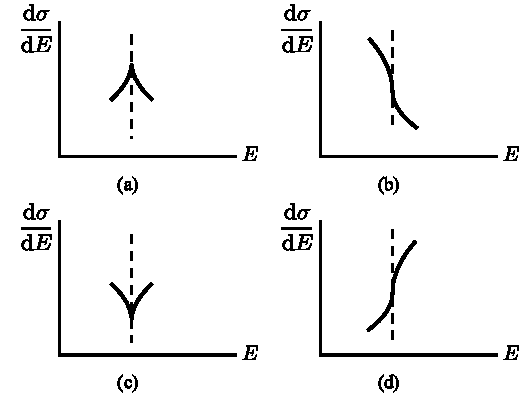
\includegraphics[width=9cm]{fig50.pdf}\\[0.3em]{\small 图 50}\end{minipage}\par\nopagebreak

(147.9)对 $\mathrm{d}o$ 积分时，第二项的积分贡献只能来自 $f_{\text{阈}}(\theta)$ 的各向同性部分，即弹性散射的 $s$ 分波振幅 $\left(\mathrm{e}^{2\mathrm{i}\delta_0}-1\right)/2\mathrm{i}k_{\text{阈}}$.从而得阈值附近的弹性散射总截面
\begin{equation}
  \sigma=\sigma_{\text{阈}}-2A\sqrt{|E-E_{\text{阈}}|}
  \times\left\{\begin{array}{ll}
    \sin^2\delta_0, & E>E_{\text{阈}},\\[0.2em]
    \sin\delta_0\cos\delta_0, & E<E_{\text{阈}}.
  \end{array}\right.
\end{equation}
对于正的和负的 $\sin\delta_0\cos\delta_0$，上式分别具有图50中(a)或(b)的形状.

由此可知，反应阈的存在使得弹性散射截面对能量的依赖关系中出现一个特征奇点.如果粒子具有自旋，公式当然会有定量方面的差别，但是这种效应的一般特性仍然不变\footnote{自旋不等于零时，$s$ 态中的 $A'+B'$ 系统可以具有不等于零的总角动量，因而 $A+B$ 系统可以具有不同的轨道态.}.如果阈值以下除了弹性散射外还有别的反应，那么在该反应的截面中也将出现相应的奇点.这些截面都在 $E=E_{\text{阈}}$ 处具有一个奇点，并在 $E=E_{\text{阈}}$ 附近是 $\sqrt{|E-E_{\text{阈}}|}$ 的线性函数，这个函数在阈值上下具有不同的斜率.

在辐射出一个带正电荷的粒子的核反应中，我们碰到了反应产物（粒子 $A'$，$B'$）间具有库仑斥力的情形.在这种情形下，当 $v'\to0$（即 $E\to E_{\text{阈}}$）时，反应截面以及这个截面对能量的所有微商都指数式地趋于零，并在其它过程的截面中没有奇点.

最后，我们来考虑生成两个电荷相异的慢粒子的反应，因而粒子间具有库仑引力.这种反应的截面通过细致平衡原理与两个相吸慢粒子反应的截面式(143.6)相联系.因此当 $v'\to0$ 时，该截面趋向常数极限值：
\begin{equation}
  v'\to0,\qquad \sigma_r=\text{常数},
\end{equation}
亦即通过阈值时反应截面突然具有某一有限值.

现在来阐明这种反应的弹性散射截面在阈值附近的奇点性质（А.~И.~Базь，1959），但它不可能像不带电粒子那样根据阈值以上的已知规律(147.11)用前面的简单办法直接地求得.与后一种情况相比较，现在的情况由于下列事实而复杂化了：$A'+B'$ 系统在近阈区（$E<E_{\text{阈}}$）具有束缚态，它们对应于库仑引力场中的离散能级.从能量角度看来，这些态可以在粒子 $A$ 和 $B$ 的碰撞中形成，但由于弹性散射的可能性，它们只能是准定态.然而，它们的存在必然会在阈值以下的弹性散射中引起与布赖特-维格纳共振相类似的共振效应.

为了解决上述问题，我们来研究描述碰撞过程的波函数的结构.与两道的存在相一致，相互作用粒子系统的薛定谔方程具有在整个位形空间内为有限的两个独立解，令 $\psi_1$ 和 $\psi_2$ 代表这两个任意选定和任意归一化的解.我们可以把这两个函数线性组合起来用以描述其中一道为输入道情形时的散射，令 $a$ 和 $b$ 分别代表粒子对为 $A,B$ 和 $A',B'$ 的两个道，并令 $\psi=\alpha_1\psi_1+\alpha_2\psi_2$ 对应于输入道 $a$ 的情形，它描述粒子 $A$ 和 $B$ 的弹性散射以及反应 $A+B\to A'+B'$.在反应阈附近，系数 $\alpha_1$ 和 $\alpha_2$ 显著地依赖于小动量 $k_b$，而任选的函数 $\psi_1$ 和 $\psi_2$ 在 $k_b=0$ 处没有奇点.

在远距离处，函数 $\psi$ 必须表为两项之和，它们对应于 $a$ 和 $b$ 道中粒子对的运动.这两项都等于粒子的“内部”函数及其相对运动波函数的乘积\footnote{规律(147.11)不但对总截面成立，而且对各种 $l$ 的分波截面也成立，参考 §143 末尾.下面讨论的奇点因而也为所有的分波截面所具有.它的性质完全可从下面给出的对 $l=0$ 情形的处理中明显看出.为简洁计，相应的分波振幅中的指标 0 将省略掉.}，后一种函数在 $a$ 道中呈 $R_a^{-}-S_{aa}R_a^{+}$ 形式，在 $b$ 道中呈 $-S_{ab}R_b^{+}$ 形式，其中 $R^{+}$ 和 $R^{-}$ 是相应道的出射和入射波.在远大于短程力的作用距离同时远小于 $1/k_b$ 的距离 $r_0$ 处，这些函数（及其导数）应该和“反应带”内的波函数 $\psi$ 算出的数值衔接起来.衔接条件如下式所示
\begin{equation*}
\begin{aligned}
  &\alpha_1a_1+\alpha_2a_2=\left(R_a^{-}-S_{aa}R_a^{+}\right)\bigr|_{r_0},\qquad
  \alpha_1b_1+\alpha_2b_2=-S_{ab}R_b^{+}\bigr|_{r_0},\\
  &\alpha_1a_1'+\alpha_2a_2'=\left(R_a^{-}-S_{aa}R_a^{+}\right)'\bigr|_{r_0},\qquad
  \alpha_1b_1'+\alpha_2b_2'=-S_{ab}R_b^{+\,\prime}\bigr|_{r_0},
\end{aligned}
\end{equation*}
式中的 $a_1,a_1',b_1,b_1',\cdots$ 是从函数 $\psi_1$ 和 $\psi_2$ 算出的量.按照上面的讨论，在近阈处它们可看作是一些和 $k_b$ 无关的常数.把以上两对方程相除，我们得到具有两个未知数（$\alpha_1/\alpha_2$ 和 $S_{aa}$）的两个线性方程.这两个方程的系数中只包含一个“临界地”依赖于 $k_b$ 的量，即 $b$ 道中出射波的对数导数.我们把这个量定义成
\begin{equation*}
  \lambda=\frac{1}{2\pi}\left.\frac{(rR_b^{+})'}{rR_b^{+}}\right|_{r=r_0}.
\end{equation*}
我们没有必要求出这些方程的具体解答，只要注意到我们所需的量 $S_{aa}$（确定弹性散射振幅）是 $\lambda$ 的分式线性函数就足够了.阈值以下的 $\lambda$ 是实数，因为波函数 $R_b^{+}$ 是实函数，它是无穷远处具有实条件（按 $\mathrm{e}^{-\kappa_br}$ 衰减，其中 $\kappa_b=\sqrt{2m_b\left(E_{\text{阈}}-E\right)}/\hbar$）的实薛定谔方程之解.阈值以下一定有 $|S_{aa}|=1$，由此可见，这个分式线性函数 $S_{aa}(\lambda)$ 一定具有以下形式：
\begin{equation}
  S_{aa}=\frac{1+\beta\lambda}{1+\beta^{*}\lambda}\,\mathrm{e}^{2\mathrm{i}\eta},
\end{equation}
式中 $\eta$ 是一个实常数，$\beta$ 是一个复常数.

现在来求作为动量 $k_b$ 的函数的 $\lambda$ 值.由于粒子 $A$ 和 $B$ 之间作用着库仑引力，$rR_b^{+}$ 为无穷远处渐近地正比于 $\mathrm{e}^{\mathrm{i}k_br}$ 的库仑波函数.在库仑斥力场中，这个函数由 $G_0+\mathrm{i}F_0$ 给出，$G_0$ 和 $F_0$ 见(138.4)和(138.7).把式中的 $k$ 和 $r$ 同时变号，就变成了引力场情形\footnote{下面采用库仑单位. $k$ 和 $r$ 的变号在形式上相当于库仑制长度单位的变号.}.进行这种变换并算出对数导数（见§138），我们有\footnote{为了简化以后的公式，我们在大括号表达式中略去了与 $k_b$ 无关的实常数 $-\ln2r_0-2C$；这相当于不太重要地重新定义(147.12)式中的复量 $\beta$ 和实量 $\eta$.}
\begin{equation}
  \lambda=\frac{\mathrm{i}}{1-\mathrm{e}^{-2\pi/k_b}}
  -\frac{1}{\pi}\left\{\ln k_b+\frac{1}{2}\left[\psi\left(\frac{\mathrm{i}}{k_b}\right)
  +\psi\left(-\frac{\mathrm{i}}{k_b}\right)\right]\right\},
\end{equation}
式中 $k_b$ 已假定为实量，所以这个式子是属于阈值以上的区域的.当 $k_b\to0$ 时，(147.13)中的第一项趋于 $\mathrm{i}$，第二项趋于零（见§138第4个附注），因此阈值以上有
\begin{equation}
  \lambda=\mathrm{i}\quad\left(E>E_{\text{阈}}\right).
\end{equation}
把 $k$ 改成 $\mathrm{i}\kappa$ 后，就过渡到阈值以下的区域，当 $\kappa\to0$ 时由(147.13)式得\footnote{(147.13)中的第一项给出 $-\dfrac{1}{2}\cot(\pi/\kappa_b)+\dfrac{1}{2}\mathrm{i}$，(147.13)的大括号内的部分趋于 $\dfrac{1}{2}\pi\cot(\pi/\kappa_b)+\dfrac{1}{2}\mathrm{i}\pi$，其中应用了公式 $\psi(x)-\psi(-x)=-\pi\cot\pi x-1/x$.（它可从熟知公式 $\Gamma(x)\Gamma(-x)=-\pi/x\sin\pi x$ 的对数导数求出）和 $x\to\infty$ 时的极限表式
\begin{equation*}
  \psi(x)\approx\ln x-1/2x.
\end{equation*}}
\begin{equation}
  \lambda=-\cot(\pi/\kappa_b)\quad\left(E<E_{\text{阈}}\right)
\end{equation}
这些公式解决了所考虑的问题.弹性散射截面为
\begin{equation*}
  \sigma_e=\pi k_a^{-2}\,|S_{aa}-1|^2.
\end{equation*}
阈值以上有：
\begin{equation}
  S_{aa}=\frac{1+\mathrm{i}\beta}{1+\mathrm{i}\beta^{*}}\,\mathrm{e}^{2\mathrm{i}\eta}
  \quad\left(E>E_{\text{阈}}\right).
\end{equation}
和反应截面一样，散射截面在这个区域内是常数.条件 $|S_{aa}|<1$ 意味着 $\operatorname{Im}\beta>0$.阈值以下有
\begin{equation}
  S_{aa}=\mathrm{e}^{2\mathrm{i}\eta}\,
  \frac{\beta-\tan(\pi/\kappa_b)}{\beta^{*}-\tan(\pi/\kappa_b)}.
\end{equation}
这个表式具有无穷多个共振，其密度向着 $E=E_{\text{阈}}$ 点增长，这些共振能量等于下式的根：
\begin{equation*}
  S_{aa}=-1,\ \text{即}\ \operatorname{Re}\left[\mathrm{e}^{2\mathrm{i}\eta}
  \left(\beta-\tan(\pi/\kappa_b)\right)\right]=0;
\end{equation*}
由于短程力的存在，这些能级相对于纯库仑能级（它们是 $\tan(\pi/\kappa_b)=0$ 的根）而言略有移动.当能量 $E$ 趋近于阈值时，弹性散射截面在零和 $4\pi/k_a^2$ 之间振荡，如图51所示.出现共振结构的整个阈下区的宽度，由第一库仑能级的能量值所确定\footnote{近阈反应的另一个有趣情形是原子被一个电子所电离，该电子的能量只是略大于该原子的第一电离能.这些条件下的碰撞过程可以看作是准经典的，但由于末态中存在着三个带电粒子而使问题极大地复杂化了.这个难题的普遍解由 G.~H.~Wannier（Physical Review 90, 817, 1953）给出.我们发现，一个中性原子的电离概率正比于 $(E-I)^{\alpha}$，其中 $\alpha=\dfrac{1}{4}\sqrt{91/3-1}=1.13$，$E-I$ 是电子的超过电离阈值的能量.}.

\par\nopagebreak\noindent\begin{minipage}{\linewidth}\centering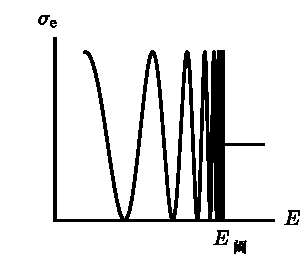
\includegraphics[width=4.8cm]{fig51.pdf}\\[0.3em]{\small 图 51}\end{minipage}\par\nopagebreak

\section{快电子和原子的非弹性碰撞}

快电子和原子间的非弹性碰撞，可用§139中对弹性碰撞的同样方式，用玻恩近似加以研究\footnote{§148—§150 中大部分结果是由 H.~A.~Bethe（1930）得到的.}.玻恩近似的适用条件仍和以前一样，入射电子的速度必须远大于原子中电子的速度，碰撞中的能量损失可以是任意值.如果电子失去了它的相当大一部分能量，原子被电离，这些能量被转移到其中的一个电子身上.可是，我们总可以把碰撞后具有较大速度的那个电子看作散射电子，这样，如果入射电子速度很大，则散射电子的速度也很大.

正如早已指出的，在一个电子和一个原子的碰撞中，质心静止的坐标系可以认为与原子静止的坐标系一致，而后一坐标系正是下面实际上要采用的.

非弹性碰撞伴有原子的内态变化.该原子可能从基态跳到某一个离散谱或连续谱的激发态，后一种情形意味着原子的电离.推导一般公式时，我们可以把这两种情形合在一起考虑.

我们先从连续谱状态之间跃迁概率的一般公式出发（和§126中一样），把它应用到具有入射电子和原子的系统.令 $\boldsymbol{p},\boldsymbol{p}'$ 为入射电子在碰撞前后的动量，$E_0,E_n$ 为原子的相应能量.至于跃迁概率，(126.9)式换成
\begin{equation}
  \mathrm{d}w_n=\frac{2\pi}{\hbar}
  \left|\left\langle n,\boldsymbol{p}'|U|0,\boldsymbol{p}\right\rangle\right|^2
  \delta\left(\frac{p'^2-p^2}{2m}+E_n-E_0\right)
  \frac{\mathrm{d}^3p'}{(2\pi\hbar)^3},
\end{equation}
式中的矩阵元是入射电子和原子间以下相互作用能的矩阵元：
\begin{equation*}
  U=\frac{Ze^2}{r}-\sum_{a=1}^{Z}\frac{e^2}{|\boldsymbol{r}-\boldsymbol{r}_a|},
\end{equation*}
式中 $\boldsymbol{r}$ 是入射电子的径矢，$\boldsymbol{r}_a$ 是原子中电子的径矢，原点位于原子核处，$m$ 是电子质量.

电子波函数 $\psi_p,\psi_{p'}$ 由以前的(126.10)(126.11)式确定，此时 $\mathrm{d}w$ 就是碰撞截面 $\mathrm{d}\sigma$.我们把初态和末态原子波函数记作 $\psi_0$ 和 $\psi_n$.如果原子的末态属于离散谱，则 $\psi_n$（和 $\psi_0$ 一样）按通常方式归一化.反之，如果原子进入连续谱的一个态，波函数应按确定该态的参量 $\nu$ 的δ函数归一化（例如，这些参量可以是原子的能量，以及电离时离开原子的那个电子的动量的各分量），由此求出的截面给出了原子碰撞到参量值介于 $\nu$ 和 $\nu+\mathrm{d}\nu$ 区间内的连续谱态时的概率.

(148.1)对绝对值 $p'$ 积分后得
\begin{equation*}
  \mathrm{d}\sigma_n=\frac{mp'}{4\pi^2\hbar^4}
  \left|\left\langle n\boldsymbol{p}'|U|0\boldsymbol{p}\right\rangle\right|^2\mathrm{d}o',
\end{equation*}
式中的 $p'$ 由能量守恒律确定：
\begin{equation}
  \frac{1}{2m}\left(p^2-p'^2\right)=E_n-E_0.
\end{equation}
把(126.10)，(126.11)式的电子波函数代入矩阵元中，得
\begin{equation}
  \mathrm{d}\sigma_n=\frac{m^2}{4\pi^2\hbar^4}\,\frac{p'}{p}
  \left|\iint U\mathrm{e}^{-\mathrm{i}\boldsymbol{q}\cdot\boldsymbol{r}}\psi_n^{*}\psi_0\,\mathrm{d}\tau\,\mathrm{d}V\right|^2\mathrm{d}o\footnotemark
\end{equation}
\footnotetext{这个公式是微扰论的一般结果，不但适用于电子和原子的碰撞，也适用于两个粒子的任何非弹性碰撞，确定了质心为静止的坐标系中的散射截面（$m$ 是这两个粒子的折合质量）.}
式中 $\mathrm{d}\tau=\mathrm{d}V_1\mathrm{d}V_2\cdots\mathrm{d}V_Z$ 是原子中 $Z$ 个电子的位形空间的体积元，我们略去了 $\mathrm{d}o$ 上的撇号.当 $n=0$ 和 $p=p'$ 时，(148.3)变成弹性散射截面公式.

由于函数 $\psi_n$ 与 $\psi_0$ 正交，$U$ 中的原子核作用项 $Ze^2/r$ 对 $\tau$ 积分后等于零.因此对非弹性碰撞有
\begin{equation}
  \mathrm{d}\sigma_n=\frac{m^2}{4\pi^2\hbar^4}\,\frac{p'}{p}\sum_a
  \left|\iint\frac{e^2}{|\boldsymbol{r}-\boldsymbol{r}_a|}\,
  \mathrm{e}^{-\mathrm{i}\boldsymbol{q}\cdot\boldsymbol{r}}\psi_n^{*}\psi_0\,\mathrm{d}\tau\,\mathrm{d}V\right|^2\mathrm{d}o.
\end{equation}
对 $V$ 的积分可按§139进行.而积分
\begin{equation*}
  \varphi_q(\boldsymbol{r}_a)=\int\frac{\mathrm{e}^{-\mathrm{i}\boldsymbol{q}\cdot\boldsymbol{r}}}
  {|\boldsymbol{r}-\boldsymbol{r}_a|}\,\mathrm{d}V
\end{equation*}
在形式上等同于密度分布为 $\rho=\delta(\boldsymbol{r}-\boldsymbol{r}_a)$ 的空间电荷在 $\boldsymbol{r}$ 点处的势的傅里叶分量，因此(139.1)式给出
\begin{equation}
  \varphi_q(\boldsymbol{r}_a)=\frac{4\pi}{q^2}\,\mathrm{e}^{-\mathrm{i}\boldsymbol{q}\cdot\boldsymbol{r}_a}.
\end{equation}
将此式代入(148.4)，最后得到以下非弹性碰撞截面的一般表式：
\begin{equation}
  \mathrm{d}\sigma_n=\left(\frac{e^2m}{\hbar^2}\right)^2\frac{4k'}{kq^4}
  \left|\left\langle n\left|\sum_a\mathrm{e}^{-\mathrm{i}\boldsymbol{q}\cdot\boldsymbol{r}_a}\right|0\right\rangle\right|^2\mathrm{d}o,
\end{equation}
式中的矩阵元是对原子波函数而言的，我们引进了波矢量 $\boldsymbol{k}'=\boldsymbol{p}'/\hbar$，$\boldsymbol{k}=\boldsymbol{p}/\hbar$ 代替了动量.这个公式给出了电子被散射到立体角元 $\mathrm{d}o$ 内而原子跃迁到第 $n$ 个激发态时的碰撞概率.矢量 $-\hbar\boldsymbol{q}$ 是电子在碰撞中给予原子的动量.

为计算方便计，最好把截面中的立体角元改成矢量 $\boldsymbol{q}$ 的绝对值的元 $\mathrm{d}q$.矢量 $\boldsymbol{q}$ 是由 $\boldsymbol{q}=\boldsymbol{k}'-\boldsymbol{k}$ 定义的，其绝对值为
\begin{equation}
  q^2=k^2+k'^2-2kk'\cos\vartheta.
\end{equation}
因此，给定了 $k,k'$，亦即给定了电子的能量损失后，有
\begin{equation}
  q\,\mathrm{d}q=kk'\sin\vartheta\,\mathrm{d}\vartheta=\frac{kk'}{2\pi}\,\mathrm{d}o,
\end{equation}
从而(148.6)式可写成
\begin{equation}
  \mathrm{d}\sigma_n=8\pi\left(\frac{e^2}{\hbar v}\right)^2\frac{\mathrm{d}q}{q^3}
  \left|\left\langle n\left|\sum_a\mathrm{e}^{-\mathrm{i}\boldsymbol{q}\cdot\boldsymbol{r}_a}\right|0\right\rangle\right|^2.
\end{equation}
矢量 $\boldsymbol{q}$ 在以下的计算中起着重要的作用.让我们较详细地考察一下它和散射角 $\vartheta$ 以及碰撞中的能量转移 $E_n-E_0$ 的关系.下面将看到，最重要的碰撞是散射角很小（$\vartheta\ll1$），能量转移远小于入射电子能量 $E=\frac{1}{2}mv^2$ 的碰撞：$E_n-E_0\ll E$.这种情形下 $k-k'$ 的值也很小（$k-k'\ll k$），而且
\begin{equation*}
  E_n-E_0=\frac{\hbar^2}{2m}\left(k^2-k'^2\right)
  \approx\frac{\hbar^2}{m}k(k-k')=\hbar v(k-k').
\end{equation*}
由于 $\vartheta$ 很小，从(148.7)式得
\begin{equation*}
  q^2\approx(k-k')^2+(k\vartheta)^2,
\end{equation*}
最后有
\begin{equation}
  q=\sqrt{\left(\frac{E_n-E_0}{\hbar v}\right)^2+(k\vartheta)^2}.
\end{equation}
$q$ 的极小值为
\begin{equation}
  q_{\mathrm{min}}=\frac{E_n-E_0}{\hbar v}.
\end{equation}
在小角度范围内，我们还可以进一步划分成不同的区域，这取决于小量 $\vartheta$ 和 $v_0/v$ 之间的关系，此处 $v_0$ 具有原子中电子速度的数量级.如果我们考虑的能量转移具有原子中电子能量 $\varepsilon_0$ 的数量级（$E_n-E_0\sim\varepsilon_0\sim mv_0^2$），则当 $(v_0/v)^2\ll\vartheta\ll1$ 时有
\begin{equation}
  q=k\vartheta=(mv/\hbar)\,\vartheta;
\end{equation}
(148.10)式根号中的第一项与第二项相比可以略去.在这个角度范围内，$q$ 因而和能量转移无关.当 $\vartheta\ll1$ 时，$q$ 既可以大于也可以小于 $1/a_0$（$a_0$ 具有原子线度的数量级）.在对能量转移作出同样的假定下，我们有
\begin{equation}
  \vartheta\sim v_0/v\ \text{时},\ \ qa_0\sim1.
\end{equation}
现在把一般公式(148.9)应用于小的 $q$（$qa_0\ll1$，即 $\vartheta\ll v_0/v$）.这种情形下可把指数因子展成 $\boldsymbol{q}$ 的幂级数：
\begin{equation*}
  \mathrm{e}^{-\mathrm{i}\boldsymbol{q}\cdot\boldsymbol{r}_a}\approx1-\mathrm{i}\boldsymbol{q}\cdot\boldsymbol{r}_a=1-\mathrm{i}qx_a,
\end{equation*}
我们选择了 $x$ 轴沿矢量 $\boldsymbol{q}$ 的坐标系.上式代入(148.9)时，由于波函数 $\psi_0$ 和 $\psi_n$ 的正交性，含1之项等于零，我们就得
\begin{equation}
  \mathrm{d}\sigma_n=8\pi\left(\frac{e}{\hbar v}\right)^2\frac{\mathrm{d}q}{q}\,
  |\langle n|d_x|0\rangle|^2
  =\left(\frac{2e}{\hbar v}\right)^2|\langle n|d_x|0\rangle|^2\,\frac{\mathrm{d}o}{\vartheta^2},
\end{equation}
式中 $d_x=e\sum_ax_a$ 是原子的偶极矩分量.我们看到，截面（对小的 $q$）是由与原子的状态变化相对应的那个偶极矩跃迁矩阵元的模量平方给出的.\footnote{物理上通常感兴趣的截面 $\mathrm{d}\sigma_n$，是对末态原子角动量的所有空间取向求和并对初态角动量的所有空间取向求平均以后的截面.经过这样的求和及求平均以后，
\begin{equation*}
  |\langle n|d_x|0\rangle|^2
\end{equation*}
和 $x$ 轴的方向无关.}

但有可能出现这样的情况，由于选择定则，对所考虑的跃迁讲来偶极矩矩阵元都等于零（禁戒跃迁），这时 $\mathrm{e}^{-\mathrm{i}\boldsymbol{q}\cdot\boldsymbol{r}_a}$ 还需展至下一项，我们得
\begin{equation}
  \mathrm{d}\sigma_n=2\pi\left(\frac{e^2}{\hbar v}\right)^2
  \left|\left\langle n\left|\sum_ax_a^2\right|0\right\rangle\right|^2q\,\mathrm{d}q.
\end{equation}
现在来考虑 $q$ 很大（$qa_0\gg1$）的相反极端情形.如果 $q$ 很大，这意味着原子接受的动量远大于原子中电子原有的内禀动量.从物理上考虑这是很明显的：在这种情形下，我们可以把原子中电子看作是自由的，而和原子的碰撞可以看作是入射电子与原子中原为静止的电子的弹性碰撞.这一点也可从普遍公式(148.9)看出来：当 $q$ 很大时，矩阵元中的被积式含有急剧振荡因子 $\mathrm{e}^{-\mathrm{i}\boldsymbol{q}\cdot\boldsymbol{r}_a}$，如果 $\psi_n$ 中不含类似的因子，这个积分差不多等于零.这样的 $\psi_n$ 函数对应于一个电离原子，辐射出一个动量为 $-\hbar\boldsymbol{q}=\boldsymbol{p}-\boldsymbol{p}'$ 的电子，这个动量相当于两个自由电子碰撞时由动量守恒律所给出的动量.

具有大动量转移的碰撞中，入射电子和原子电子有可能获得差不多大小的末速度，与相碰粒子的全同性有关的交换作用开始变得重要起来，尽管普遍公式(148.9)中并没有计及这一点.有交换的快电子散射截面由(137.9)式给出，这个公式采用的是碰撞前一个电子为静止的坐标系.对快电子讲来，(137.9)式最后一项中的余弦函数可以取作1.乘以原子中的电子数 $Z$ 以后，即得一个电子和一个原子碰撞的以下截面式：
\begin{equation}
  \mathrm{d}\sigma=4Z\left(\frac{e^2}{mv^2}\right)^2
  \left[\frac{1}{\sin^4\vartheta}+\frac{1}{\cos^4\vartheta}
  -\frac{1}{\sin^2\vartheta\cos^2\vartheta}\right]\cos\vartheta\,\mathrm{d}o,
\end{equation}
为方便计，此式中的散射角最好用碰撞后电子具有的能量来表达.我们知道，能量为 $E=\frac{1}{2}mv^2$ 的粒子和同质量的静止粒子相碰后，所得的粒子能量分别为
\begin{equation*}
  \varepsilon=E\sin^2\vartheta,\qquad E-\varepsilon=E\cos^2\vartheta.
\end{equation*}
为了求出有关 $\mathrm{d}\varepsilon$ 区间的截面，我们按关系式
\begin{equation*}
  \cos\vartheta\,\mathrm{d}o=2\pi\sin\vartheta\cos\vartheta\,\mathrm{d}\vartheta
  =(\pi/E)\,\mathrm{d}\varepsilon,
\end{equation*}
把 $\mathrm{d}o$ 化成 $\mathrm{d}\varepsilon$.代入(148.16)即得最后表式
\begin{equation}
  \mathrm{d}\sigma_{\varepsilon}=\pi Ze^4\left[\frac{1}{\varepsilon^2}
  +\frac{1}{(E-\varepsilon)^2}-\frac{1}{\varepsilon(E-\varepsilon)}\right]\frac{\mathrm{d}\varepsilon}{E}.
\end{equation}
如果能量 $\varepsilon$ 和 $E-\varepsilon$ 中有一个远小于另一个，上式三项中只有一项（第一或第二项）是重要的.这是可以预料的，因为当两个电子的能量相差很大时，交换作用不再重要，它应回到熟知的卢瑟福公式\footnote{对于正电子和原子的碰撞不存在交换效应，卢瑟福公式
\begin{equation*}
  \mathrm{d}\sigma_{\varepsilon}=\frac{\pi Ze^4}{E}\,\frac{\mathrm{d}\varepsilon}{\varepsilon^2}
\end{equation*}
对所有的 $g\gg1/a_0$ 成立.}.

微分截面对所有角度积分（或对 $q$ 积分）后给出把原子激发到给定态的总截面 $\sigma_n$.$\sigma_n$ 与入射电子速度的关系，是和偶极矩的相应跃迁矩阵元是否存在具有密切的关系.我们先假定这个矩阵元不等于零.于是当 $q$ 小时，$\mathrm{d}\sigma_n$ 由(148.14)式给出，而且我们看到，当 $q$ 减小时对 $q$ 的积分是对数发散的.另一方面，在大 $q$ 的区域内，当 $q$ 增大时截面（对一给定的能量转移 $E_n-E_0$）指数式地减小，这是因为(148.9)矩阵元的被积函数中存在着一个（早已指出的）剧烈振荡因子.由此可见，对 $q$ 积分时 $q$ 值小的区域起着主要作用，我们可把积分范围限制在从(148.11)式的极小值开始到数量级为 $1/a_0$ 的某个值为止.

结果得
\begin{equation}
  \sigma_n=8\pi\left(\frac{e}{\hbar v}\right)^2|\langle n|d_x|0\rangle|^2
  \ln\left(\beta_n\,\frac{v\hbar}{e^2}\right),
\end{equation}
其中 $\beta_n$ 是一个量纲为1的常数，我们不可能算出它的一般形式\footnote{我们假定了 $E_n-E_0$ 具有原子中电子能量 $\varepsilon_0$ 的数量级.对于更大的能量转移（$E_n-E_0\sim E\gg\varepsilon_0$），(148.14)和(148.18)仍不能适用，因为此时的偶极矩矩阵元变得很小，不能只取 $q$ 的幂级数展式的第一项.}.

另一方面，如果偶极矩矩阵元对于所考虑的跃迁讲来等于零，那么对 $q$ 的积分无论对小的 $q$（可从(148.15)式看出）以及对大的 $q$ 都是很快地收敛的.积分中 $q$ 的最重要区域为 $q\sim1/a_0$，这时不可能得到普遍的定量公式，我们只能推出这样的结论：$\sigma_n$ 将和速度的平方成反比：
\begin{equation}
  \sigma_n=\frac{\text{常数}}{v^2}.
\end{equation}
这可从普遍公式(148.9)直接看到，按该式当 $q\sim1/a_0$ 时 $\mathrm{d}\sigma_n$ 将和 $1/v^2$ 成正比.

我们来求散射到某一给定立体角元而不管原子进入哪个态的非弹性散射截面 $\mathrm{d}\sigma_r$.为此，需要把(148.9)式对所有 $n\neq0$ 的态求和，也就是对基态以外的所有原子态（包括离散谱和连续谱）求和.我们不去考虑大角度区间和小角度区间，而假定 $(v_0/v)^2\ll\vartheta\ll1$，于是按(148.12)，$q$ 和能量转移值无关\footnote{(148.9)式的求和也对 $E_n-E_0\gg\varepsilon_0$ 的态进行，此时(148.12)式不再成立.但对具有大能量转移的跃迁来讲，有效截面比较小，这些项在求和式中并不重要.所加的条件 $\vartheta\ll1$ 使我们可以不必考虑交换效应.}.

后一种情况使我们很易算出非弹性碰撞的总截面，亦即求和式
\begin{equation}
\begin{aligned}
  \mathrm{d}\sigma_r&=\sum_{n\neq0}\mathrm{d}\sigma_n
  =8\pi\left(\frac{e^2}{\hbar v}\right)^2\sum_{n\neq0}
  \left|\left\langle n\left|\sum_a\mathrm{e}^{-\mathrm{i}\boldsymbol{q}\cdot\boldsymbol{r}_a}\right|0\right\rangle\right|^2
  \frac{\mathrm{d}q}{q^3}=\\
  &=\left(\frac{2e^2}{mv^2}\right)^2\sum_{n\neq0}
  \left|\left\langle n\left|\sum_a\mathrm{e}^{-\mathrm{i}\boldsymbol{q}\cdot\boldsymbol{r}_a}\right|0\right\rangle\right|^2
  \frac{\mathrm{d}o}{\vartheta^4}.
\end{aligned}
\end{equation}
为此我们注意到，根据矩阵乘法规则，对任意一个量 $f$ 有
\begin{equation*}
  \sum_n|f_{0n}|^2=\sum_nf_{0n}(f_{0n})^{*}
  =\sum_nf_{0n}(f^{+})_{n0}=(ff^{+})_{00}
\end{equation*}
上式是对所有的 $n$ 求和，包括 $n=0$.因而
\begin{equation}
  \sum_{n\neq0}|f_{0n}|^2=\sum_n|f_{0n}|^2-|f_{00}|^2=(ff^{+})_{00}-|f_{00}|^2.
\end{equation}
把此式应用于 $f=\sum_a\mathrm{e}^{-\mathrm{i}\boldsymbol{q}\cdot\boldsymbol{r}_a}$，我们有
\begin{equation}
  \mathrm{d}\sigma_r=\left(\frac{2e^2}{mv^2}\right)^2
  \left\{\left\langle\left|\sum_a\mathrm{e}^{-\mathrm{i}\boldsymbol{q}\cdot\boldsymbol{r}_a}\right|^2\right\rangle
  -\left|\left\langle\sum_a\mathrm{e}^{-\mathrm{i}\boldsymbol{q}\cdot\boldsymbol{r}_a}\right\rangle\right|^2\right\}
  \frac{\mathrm{d}o}{\vartheta^4},
\end{equation}
式中 $\langle\cdots\rangle$ 代表对原子基态求平均（取00对角矩阵元）.根据定义，平均值
$\left\langle\sum_a\mathrm{e}^{-\mathrm{i}\boldsymbol{q}\cdot\boldsymbol{r}_a}\right\rangle$
就是基态原子的原子形状因子 $F(q)$.大括号内的第一项可写成
\begin{equation*}
  \left|\sum_{a=1}^{Z}\mathrm{e}^{-\mathrm{i}\boldsymbol{q}\cdot\boldsymbol{r}_a}\right|^2
  =Z+\sum_{a\neq b}\mathrm{e}^{\mathrm{i}\boldsymbol{q}\cdot(\boldsymbol{r}_a-\boldsymbol{r}_b)},
\end{equation*}
从而得一般公式
\begin{equation}
  \mathrm{d}\sigma_r=\left(\frac{2e^2}{mv^2}\right)^2
  \left\{Z-F^2(q)+\left\langle\sum_{a\neq b}
  \mathrm{e}^{\mathrm{i}\boldsymbol{q}\cdot(\boldsymbol{r}_a-\boldsymbol{r}_b)}\right\rangle\right\}
  \frac{\mathrm{d}o}{\vartheta^4}.
\end{equation}
当 $q$ 很小可按 $q$ 的幂展开（$v_0/v\ll qa_0\ll1$，相当于角度 $(v_0/v)^2\ll\vartheta\ll v_0/v$）时，此式可大为化简.为方便计，我们不去展开(148.23)式，而把(148.14)式的 $\mathrm{d}\sigma_n$ 重新对 $n$ 求和.利用 $f=d_x$ 的(148.21)式并记得 $\langle d_x\rangle=0$，求和后得
\begin{equation}
  \mathrm{d}\sigma_r=\left(\frac{2e}{\hbar v}\right)^2\langle d_x^2\rangle\frac{\mathrm{d}o}{\vartheta^2}.
\end{equation}
把上式和小角度弹性散射截面式(139.5)比较一下是有意义的，后者和 $\vartheta$ 无关，散射到 $\mathrm{d}o$ 立体角元内的非弹性截面则随 $\vartheta$ 的减小而按 $1/\vartheta^2$ 的规律增长.

对于 $v_0/v\ll\vartheta\ll1$（因而 $qa_0\gg1$）范围内的 $\vartheta$ 角，(148.23)大括号内的第二和第三项都很小，我们简单地有
\begin{equation}
  \mathrm{d}\sigma_r=Z\left(\frac{2e^2}{mv^2}\right)^2\frac{\mathrm{d}o}{\vartheta^4}
\end{equation}
也就是对 $Z$ 个原子电子的卢瑟福散射（没有交换作用）.我们记得，对于弹性散射有(139.6)式，它不是和 $Z$ 而是和 $Z^2$ 成正比.

最后，对角度积分后，我们得到对所有的角度以及对原子的任意激发而言的非弹性散射总截面 $\sigma_r$.和计算(148.18)式的 $\sigma_n$ 完全一样，可得
\begin{equation}
  \sigma_r=8\pi\left(\frac{e}{\hbar v}\right)^2\langle d_x^2\rangle
  \ln\left(\beta\,\frac{v\hbar}{e^2}\right).
\end{equation}

% 【脚注代理】原书 p572：“习\ 题”标题本身系圈码①（脚注“所有题都采用原子单位.”）。
% xiti 环境标题系固定排版，此处局部展开环境以便把脚注按原书系于标题
% （对应的 \end{xiti} 一并展开为 \par，见下）。
\par\medskip\noindent{\heiti 习\ 题\footnote{所有题都采用原子单位.}}\par\smallskip\noindent

\noindent{\heiti 习题1}\quad 求快电子被氢原子（处于基态）非弹性散射的角分布
（$\left(v_0/v\right)^2\ll\vartheta\ll1$）.

解：对氢原子而言，(148.23)大括号内的第三项等于零，而原子形状因子 $F(q)$ 已在§139例题中算出.把它代入得
\begin{equation*}
  \mathrm{d}\sigma_r=\frac{4}{v^4\vartheta^4}
  \left[1-\frac{1}{\left(1+\dfrac{v^2\vartheta^2}{4}\right)^4}\right]\mathrm{d}o.
\end{equation*}

\noindent{\heiti 习题2}\quad 基态氢原子受电子碰撞而激发到第 $n$ 个离散谱能级（$n$ 是主量子数），求微分截面.

解：最好用抛物坐标计算矩阵元.取 $z$ 轴沿矢量 $\boldsymbol{q}$ 的方向，此时有
$\mathrm{e}^{\mathrm{i}\boldsymbol{q}\cdot\boldsymbol{r}}=\mathrm{e}^{\mathrm{i}qz}
=\mathrm{e}^{\mathrm{i}q(\xi-\eta)/2}$.基态波函数呈
$\psi_{000}=\pi^{-1/2}\mathrm{e}^{-(\xi+\eta)/2}$ 形式.仅当跃迁到 $m=0$ 的态时矩阵元才不等于零.这种态的波函数为
\begin{equation*}
  \psi_{n_1n_20}=\frac{1}{\sqrt{\pi}\,n^2}\,
  \mathrm{e}^{-\frac{\xi+\eta}{2n}}
  \mathrm{F}\left(-n_1,1,\frac{\xi}{n}\right)
  \mathrm{F}\left(-n_2,1,\frac{\eta}{n}\right)
\end{equation*}
（$n=n_1+n_2+1$）.所求的矩阵元由以下积分式给出：
\begin{equation*}
  \left\langle n_1n_20\left|\mathrm{e}^{\mathrm{i}\boldsymbol{q}\cdot\boldsymbol{r}}\right|000\right\rangle
  =\iint_0^{\infty}\mathrm{e}^{\mathrm{i}\frac{q}{2}(\xi-\eta)}
  \psi_{000}\psi_{n_1n_20}\,\frac{(\xi+\eta)}{4}\,2\pi\,\mathrm{d}\xi\,\mathrm{d}\eta,
\end{equation*}
这个积分可用数学附录§f中所引的公式加以计算.结果得：
\begin{equation*}
  \left|\left\langle n_1n_20\left|\mathrm{e}^{\mathrm{i}\boldsymbol{q}\cdot\boldsymbol{r}}\right|000\right\rangle\right|^2
  =2^8n^6q^2\,\frac{\left[(n-1)^2+(qn)^2\right]^{n-3}}{\left[(n+1)^2+(qn)^2\right]^{n+3}}
  \left[(n_1-n_2)^2+(qn)^2\right],
\end{equation*}
$n_1+n_2=n-1$ 值相同的态都有相同的能量.在 $n$ 为给定的情形下，对所有可能的 $n_1-n_2$ 值求和，并把结果代入(148.9)，即得所求的截面：
\begin{equation*}
  \mathrm{d}\sigma_n=\frac{2^{11}\pi}{v^2}\,n^7
  \left[\frac{n^2-1}{3}+(qn)^2\right]
  \frac{\left[(n-1)^2+(qn)^2\right]^{n-3}}{\left[(n+1)^2+(qn)^2\right]^{n+3}}\,
  \frac{\mathrm{d}q}{q}.
\end{equation*}

\noindent{\heiti 习题3}\quad 试求氢原子第一激发态被激发的总截面.

解：公式
\begin{equation*}
  \mathrm{d}\sigma_2=\frac{2^8\pi}{v^2}\,
  \frac{\mathrm{d}q}{q\left(q^2+\dfrac{9}{4}\right)^5}
\end{equation*}
尚需对从 $q_{\mathrm{min}}=(E_2-E_1)/v=3/8v$ 到 $q_{\mathrm{max}}=2v$ 的所有 $q$ 值积分，只保留 $v$ 的最高次项.经过初等积分后结果得\footnote{对任意的 $n$ 也能算出截面.用数值计算法还可以算出被氢原子非弹性散射的总截面：
\begin{equation*}
  \sigma_r=4\pi\ln\frac{v^2}{0.160},
\end{equation*}
式中包括了以下两项贡献，即来自原子离散谱状态被激发的碰撞以及原子被电离的碰撞：
\begin{equation*}
  \sigma_{\text{激发}}=\frac{4\pi}{v^2}\times0.715\ln\left(\frac{v^2}{0.160}\right),
\end{equation*}
\begin{equation*}
  \sigma_{\text{电离}}=\frac{4\pi}{v^2}\times0.285\ln\left(\frac{v^2}{0.012}\right).
\end{equation*}}
\begin{equation*}
  \sigma_2=\frac{2^{18}\pi}{3^{10}v^2}\left(\ln4v-\frac{25}{24}\right)
  =\frac{4\pi}{v^2}\,0.555\ln\frac{v^2}{0.50}.
\end{equation*}

\noindent{\heiti 习题4}\quad 求氢原子（处于基态）电离而次级电子发射到给定方向的有效截面；次级电子的能量远小于初级电子的能量，故交换作用可以略去（H.~S.~W.~Massey，C.~Mohr，1933）.

解：初态的原子波函数为 $\psi_0=\pi^{-1/2}\mathrm{e}^{-r}$.末态的原子已电离，从中发射出的电子具有波矢量 $\boldsymbol{\kappa}$（和能量 $\varepsilon=\frac{1}{2}\kappa^2$）.这个态由(136.9)的函数 $\psi_{\kappa}^{(-)}$ 描写，其中的出射部分（在无穷远处）只有沿 $\boldsymbol{\kappa}$ 方向传播的一个平面波.$\psi_{\kappa}^{(-)}$ 函数已按 $\boldsymbol{\kappa}/2\pi$ 空间的δ函数归一化，因此由它算出的截面是对 $\mathrm{d}^3\kappa/(2\pi)^3$ 亦即 $\kappa^2\mathrm{d}\kappa\,\mathrm{d}o_{\kappa}/(2\pi)^3$ 而言的，$\mathrm{d}o_{\kappa}$ 是沿次级电子方向的立体角元.于是有
\begin{equation*}
  \mathrm{d}\sigma=\frac{4k'\kappa^2}{(2\pi)^3kq^4}\,
  \left|\left\langle\boldsymbol{\kappa}\left|\mathrm{e}^{-\mathrm{i}\boldsymbol{q}\cdot\boldsymbol{r}}\right|0\right\rangle\right|^2
  \mathrm{d}o\,\mathrm{d}o_{\kappa}\,\mathrm{d}\kappa
\end{equation*}
（$\mathrm{d}o$ 是对散射电子而言的立体角元），其中的
\begin{equation*}
  \left\langle\boldsymbol{\kappa}\left|\mathrm{e}^{-\mathrm{i}\boldsymbol{q}\cdot\boldsymbol{r}}\right|0\right\rangle
  =\int\psi_{\kappa}^{(-)*}\mathrm{e}^{-\mathrm{i}\boldsymbol{q}\cdot\boldsymbol{r}}\psi_0\,\mathrm{d}V
  =\frac{\mathrm{e}^{-\pi/2\kappa}\Gamma(1-\mathrm{i}/\kappa)}{\pi^{1/2}}\,I,
\end{equation*}
\begin{equation*}
  I=\left\{-\frac{\partial}{\partial\lambda}\int
  \exp\left(-\mathrm{i}\boldsymbol{q}\cdot\boldsymbol{r}-\mathrm{i}\kappa r-\lambda r\right)
  \mathrm{F}\left(\frac{\mathrm{i}}{\kappa},1,\mathrm{i}(\kappa r+\boldsymbol{\kappa}\cdot\boldsymbol{r})\right)
  \frac{\mathrm{d}V}{r}\right\}_{\lambda=1}.
\end{equation*}
积分时采用抛物坐标，$z$ 轴沿 $\boldsymbol{\kappa}$ 方向，$\varphi$ 角从 $(\boldsymbol{q},\boldsymbol{k})$ 平面算起：
\begin{equation*}
\begin{aligned}
  I=\bigg\{-\frac{1}{2}\frac{\partial}{\partial\lambda}
  &\int_0^{\infty}\!\!\int_0^{\infty}\!\!\int_0^{2\pi}
  \exp\bigg[-\frac{\mathrm{i}}{2}q(\xi-\eta)\cos\gamma
  +\mathrm{i}q\sqrt{\xi\eta}\sin\gamma\cos\varphi-\\
  &-\frac{\lambda}{2}(\xi+\eta)-\frac{\mathrm{i}}{2}\kappa(\xi-\eta)\bigg]
  \mathrm{F}\left(-\frac{\mathrm{i}}{\kappa},1,-\mathrm{i}\kappa\xi\right)
  \mathrm{d}\varphi\,\mathrm{d}\xi\,\mathrm{d}\eta\bigg\}_{\lambda=1},
\end{aligned}
\end{equation*}
式中 $\gamma$ 是 $\boldsymbol{\kappa}$ 和 $\boldsymbol{q}$ 的夹角.作替代 $\sqrt{\eta}\cos\varphi=u$，$\sqrt{\eta}\sin\varphi=v$ 后，很易对 $\varphi$ 和 $\eta$ 积分，积出后得
\begin{equation*}
\begin{aligned}
  \frac{I}{2\pi}=\bigg\{&\frac{\partial}{\partial\lambda}\int_0^{\infty}
  \exp\left\{\frac{-q^2\sin^2\gamma+\lambda^2+(\kappa+q\cos\gamma)^2}
  {2\left[\mathrm{i}(\kappa+q\cos\gamma)-\lambda\right]}\,\xi\right\}\times\\
  &\times\frac{\mathrm{F}\left(-\dfrac{\mathrm{i}}{\kappa},1,-\mathrm{i}\kappa\xi\right)\mathrm{d}\xi}
  {\left[\mathrm{i}(\kappa+q\cos\gamma)\xi-\lambda\right]}\bigg\}_{\lambda=1},
\end{aligned}
\end{equation*}
此处的积分可从 $\gamma=1$，$n=0$ 的(f.3)式求出.进一步的计算虽然冗长但是是初等的，结果得到以下的截面表式：
\begin{equation*}
\begin{aligned}
  \mathrm{d}\sigma&=\frac{2^8k'\kappa\left[q^2+2q\kappa\cos\gamma+(\kappa^2+1)\cos^2\gamma\right]}
  {\pi kq^2\left[q^2+2q\kappa\cos\gamma+1+\kappa^2\right]^4
  \left[(q+\kappa)^2+1\right]\left[(q-\kappa)^2+1\right]\left(1-\mathrm{e}^{-2\pi/\kappa}\right)}\times\\
  &\quad\times\exp\left(-\frac{2}{\kappa}\,\mathrm{arctan}\,\frac{2\kappa}{q^2-\kappa^2+1}\right)
  \mathrm{d}o\,\mathrm{d}o_{\kappa}\,\mathrm{d}\kappa.
\end{aligned}
\end{equation*}
对次级电子的所有发射角求积分时可用初等方法进行，结果得到辐射电子能量给定为 $\frac{1}{2}\kappa^2$ 情形下散射的角分布：
\begin{equation*}
  \mathrm{d}\sigma=\frac{2^{10}k'\kappa}{kq^2}\,
  \frac{\left[q^2+\frac{1}{3}(1+\kappa^2)\right]
  \exp\left(-\dfrac{2}{\kappa}\,\mathrm{arctan}\,\dfrac{2\kappa}{q^2-\kappa^2+1}\right)}
  {\left[(q+\kappa)^2+1\right]^3\left[(q-\kappa)^2+1\right]^3\left(1-\mathrm{e}^{-2\pi/\kappa}\right)}\,
  \mathrm{d}o\,\mathrm{d}\kappa.
\end{equation*}
$q\gg1$ 时上式在 $\kappa\approx q$ 处具有很陡的极大值；在这个极大值附近有
\begin{equation*}
  \mathrm{d}\sigma=\frac{2^5}{3\pi\kappa^4}\,
  \frac{\mathrm{d}\kappa\,\mathrm{d}o}{\left[1+(q-\kappa)^2\right]^3}.
\end{equation*}
对 $\mathrm{d}o=2\pi q\,\mathrm{d}q/k^2\cong(2\pi\kappa/k^2)\,\mathrm{d}(q-\kappa)$ 积分后，得到表式 $8\pi\,\mathrm{d}\kappa/k^2\kappa^3$，正如我们所预期的那样，它和(148.17)式中的第一项一致.
\par% 【脚注代理】上端习题块因标题带脚注局部展开了 xiti 环境，此处为其结束代码

\section{有效滞阻}

碰撞理论的应用中，计算碰撞粒子的平均能量损失极为重要.我们最好用以下的量标志这种能量损失：
\begin{equation}
  \mathrm{d}\kappa=\sum_n\left(E_n-E_0\right)\mathrm{d}\sigma_n,
\end{equation}
我们将把这个量称为（微分）有效滞阻，式中的求和当然既包括离散谱也包括连续谱，$\mathrm{d}\kappa$ 是对散射到某一给定立体角元内的情形而言的.\footnote{如果一个电子通过气体，它在各个原子上的散射是彼此独立地进行的，那么 $N\mathrm{d}\kappa$（$N$ 是单位体积内的气体原子数）就是电子在偏转到给定的立体角元的碰撞中单位路程内所损失的能量.}

快电子有效滞阻的一般公式为：
\begin{equation}
  \mathrm{d}\kappa=8\pi\left(\frac{e^2}{\hbar v}\right)^2\sum_n\left(E_n-E_0\right)
  \left|\left\langle n\left|\sum_a\mathrm{e}^{-\mathrm{i}\boldsymbol{q}\cdot\boldsymbol{r}_a}\right|0\right\rangle\right|^2
  \frac{\mathrm{d}q}{q^3},
\end{equation}
其中的 $\mathrm{d}\sigma_n$ 取自(148.9)式.正如推导(148.23)式那样，我们排除了对极小角度区域的考虑，并假定 $(v_0/v)^2\ll\vartheta\ll1$.于是 $q$ 和能量转移值无关，我们就可以算出对 $n$ 求和的一般形式.

这个算法要用到下面导出的求和定理.作为坐标函数的某个量 $f$，它的矩阵元及其对时间导数 $\dot{f}$ 的矩阵元由下式联系：
\begin{equation}
  \left(\dot{f}\right)_{0n}=-\frac{\mathrm{i}}{\hbar}\left(E_n-E_0\right)f_{0n},
\end{equation}
所以有
\begin{equation*}
\begin{aligned}
  &\sum_n\left(E_n-E_0\right)|f_{0n}|^2
  =\sum_n\left(E_n-E_0\right)f_{0n}(f_{0n})^{*}=\\
  &\qquad=\sum_n\left(E_n-E_0\right)f_{0n}(f^{*})_{n0}
  =\mathrm{i}\hbar\sum_n(\dot{f})_{0n}(f^{*})_{n0}
  =\mathrm{i}\hbar(\dot{f}f^{*})_{00}.
\end{aligned}
\end{equation*}
原子的定态波函数可以选成实函数.此时坐标函数 $f$ 的矩阵元就具有关系式 $f_{0n}=f_{n0}$，而对(149.3)式的矩阵元讲来就有相应的关系式 $(\dot{f})_{0n}=-(\dot{f})_{n0}$.因此以上的求和式还可写成以下形式：
\begin{equation*}
  \sum_n\left(E_n-E_0\right)|f_{0n}|^2
  =-\mathrm{i}\hbar\sum_n(f^{+})_{0n}(\dot{f})_{n0}
  =-\mathrm{i}\hbar(f^{+}\dot{f})_{00}.
\end{equation*}
以上两式相加后除以2，即得求和定理：
\begin{equation}
  \sum_n\left(E_n-E_0\right)|f_{0n}|^2
  =\frac{\mathrm{i}\hbar}{2}\left(\dot{f}f^{+}-f^{+}\dot{f}\right)_{00}.
\end{equation}
我们把它应用于
\begin{equation*}
  f=\sum_a\mathrm{e}^{-\mathrm{i}\boldsymbol{q}\cdot\boldsymbol{r}_a},
\end{equation*}
根据(19.2)式，$f$ 的时间微商可用以下的算符表出
\begin{equation*}
  \hat{\dot{f}}=-\frac{\hbar}{2m}\sum_a
  \left[\mathrm{e}^{-\mathrm{i}\boldsymbol{q}\cdot\boldsymbol{r}_a}(\boldsymbol{q}\cdot\nabla_a)
  +(\boldsymbol{q}\cdot\nabla_a)\mathrm{e}^{-\mathrm{i}\boldsymbol{q}\cdot\boldsymbol{r}_a}\right].
\end{equation*}
$\hat{\dot{f}}$ 和 $\hat{f}^{+}$ 的对易结果很易直接算得：
\begin{equation*}
  \hat{\dot{f}}\hat{f}^{+}-\hat{f}^{+}\hat{\dot{f}}=-\frac{\mathrm{i}\hbar}{m}q^2Z.
\end{equation*}
代入(149.4)，即得下式
\begin{equation}
  \sum_n\frac{2m}{\hbar^2q^2}\left(E_n-E_0\right)
  \left|\left\langle n\left|\sum_a\mathrm{e}^{-\mathrm{i}\boldsymbol{q}\cdot\boldsymbol{r}_a}\right|0\right\rangle\right|^2
  =Z,
\end{equation}
它已实现了我们所要求的求和计算.\footnote{推导这个公式时，我们从来没有利用过指标“0”代表原子基态，因此这个公式对任意的初态都是成立的.}

因此得到关于微分有效滞阻的公式
\begin{equation}
  \mathrm{d}\kappa=4\pi\,\frac{Ze^4}{mv^2}\,\frac{\mathrm{d}q}{q}
  =\frac{2Ze^4}{mv^2}\,\frac{\mathrm{d}o}{\vartheta^2}.
\end{equation}
它的适用范围由以下不等式给出：
\begin{equation*}
  \left(\frac{v_0}{v}\right)^2\ll\vartheta\ll1,\qquad
  \text{即}\ \frac{v_0}{v}\ll a_0q\ll\frac{v}{v_0}.
\end{equation*}
其次，当动量转移不超过某一值 $q_1$ 而 $v_0/v\ll a_0q_1\ll v/v_0$ 时，我们来求所有碰撞的总有效滞阻
\begin{equation}
  \kappa(q_1)=\sum_n\int_{q_{\mathrm{min}}}^{q_1}\left(E_n-E_0\right)\mathrm{d}\sigma_n,
\end{equation}
$q_{\mathrm{min}}$ 由(148.11)式给出.式中的积分号不能搬到 $\sum_n$ 的前面，因为 $q_{\mathrm{min}}$ 依赖于 $n$.

我们把积分区间划分成两段，从 $q_{\mathrm{min}}$ 到 $q_0$ 的一段和 $q_0$ 到 $q_1$ 的一段，其中的 $q_0$ 是 $q$ 的某个值，满足 $v_0/v\ll q_0a_0\ll1$.于是在 $q_{\mathrm{min}}$ 到 $q_0$ 的整个积分区间内，我们可用(148.14)式的 $\mathrm{d}\sigma_n$：
\begin{equation*}
  \kappa(q_0)=8\pi\left(\frac{e}{\hbar v}\right)^2\sum_n
  |\langle n|d_x|0\rangle|^2\left(E_n-E_0\right)
  \int_{q_{\mathrm{min}}}^{q_0}\frac{\mathrm{d}q}{q},
\end{equation*}
从而
\begin{equation}
  \kappa(q_0)=8\pi\left(\frac{e}{\hbar v}\right)^2\sum_n
  |\langle n|d_x|0\rangle|^2\left(E_n-E_0\right)
  \ln\frac{q_0\hbar v}{E_n-E_0}.
\end{equation}
在 $q_0$ 到 $q_1$ 的区间内，可先对 $n$ 求和，给出(149.6)式的 $\mathrm{d}\kappa$，然后对 $q$ 积分，得出
\begin{equation}
  \kappa(q_1)-\kappa(q_0)=4\pi\,\frac{Ze^4}{mv^2}\ln\frac{q_1}{q_0}.
\end{equation}
为了变换以上的表式，我们利用(149.4)得出的求和定理，在该式中令
\begin{equation*}
  \hat{f}=\frac{d_x}{e}=\sum_ax_a,\qquad
  \hat{\dot{f}}=\frac{1}{m}\sum_a\hat{p}_{xa}.
\end{equation*}
把 $\hat{f}^{+}$ 和 $\hat{\dot{f}}$ 对易（现在的 $\hat{f}^{+}$ 等于 $\hat{f}$）得出
$\hat{\dot{f}}\hat{f}^{+}-\hat{f}^{+}\hat{\dot{f}}=-\mathrm{i}\hbar Z/m$，因而\footnote{(149.5)式的附注对本式也适用.}
\begin{equation}
  \sum_nN_{0n}\equiv\sum_n\frac{2m}{e^2\hbar^2}\left(E_n-E_0\right)
  |\langle n|d_x|0\rangle|^2=Z.
\end{equation}
量 $N_{0n}$ 称为各个相应跃迁的振子强度.

我们引进原子的某个平均能量 $I$，它由下式定义
\begin{equation}
  \ln I=\frac{\sum_nN_{0n}\ln(E_n-E_0)}{\sum_nN_{0n}}
  =\frac{1}{Z}\sum_nN_{0n}\ln(E_n-E_0).
\end{equation}
然后应用(149.10)，可把(149.8)改成
\begin{equation*}
  \kappa(q_0)=\frac{4\pi Ze^4}{mv^2}\ln\left(\frac{q_0\hbar v}{I}\right).
\end{equation*}
此式和(149.9)相加，最后得
\begin{equation}
  \kappa(q_1)=\frac{4\pi Ze^4}{mv^2}\ln\left(\frac{q_1\hbar v}{I}\right).
\end{equation}
此式中只出现一个标志所给原子的常数\footnote{对氢原子，$I=0.55me^4/\hbar^2=14.9$ eV.对重原子，我们采用托马斯–费米方法计算常数 $I$，可望得到很好的精确性.很易确立这样算出的 $I$ 值如何依赖于 $Z$.在准经典情形下，多粒子系统的本征频率相当于它的能级差.原子的平均本征频率具有 $v_0/a_0$ 的数量级.由此可知，$I\sim\hbar v_0/a_0$.托马斯–费米模型中原子电子的速度和 $Z$ 的关系为 $Z^{2/3}$，而原子的线度按 $Z^{-1/3}$ 变化.可见 $I$ 必正比于 $Z$；$I=$ 常数 $\times Z$.根据实验结果发现，这个常数约为 10 eV 的数量级.}.

通过 $q_1=mv\vartheta_1/\hbar$ 用散射角 $\vartheta_1$ 表达 $q_1$，即得所有散射到 $\vartheta\leqslant\vartheta_1$ 区间内的有效滞阻：
\begin{equation}
  \kappa(\vartheta_1)=4\pi\,\frac{Ze^4}{mv^2}\ln\left(\frac{mv^2\vartheta_1}{I}\right).
\end{equation}
如果 $q_1a_0\gg1$（即 $\vartheta_1\gg v_0/v$），我们可把 $\kappa$ 表成入射电子所能给予原子的最大能量转移值的函数.我们在上节中曾经指出，$qa_0\gg1$ 时原子被电离，差不多所有的动量 $\hbar q$ 和能量都交给了一个原子电子.由于 $\hbar q$ 和 $\varepsilon$ 是一个电子的动量和能量，即有关系 $\varepsilon=\hbar^2q^2/2m$.把 $q_1^2=2m\varepsilon_1/\hbar^2$ 代入(149.12)，我们得碰撞中能量转移 $\varepsilon\leqslant\varepsilon_1$ 的有效滞阻：
\begin{equation}
  \kappa(\varepsilon_1)=\frac{2\pi Ze^4}{mv^2}\ln\left(\frac{2m\varepsilon_1v^2}{I^2}\right).
\end{equation}
最后，我们作如下的说明.原子的各个离散谱能级主要来自一个单（外层）电子的激发.即使是两个电子的激发，它所需要的能量通常足以使该原子电离.因此，在振子强度的求和式中，跃迁到离散谱态的只是数量级等于1的那一部分；而伴有电离的则构成另一部分，其数量级为 $Z$.由此可知，伴有电离的碰撞在滞阻（被重原子滞阻）中起主要作用.

\begin{xiti}

\noindent{\heiti 习题}\quad 试求一个电子被一个氢原子滞阻（$I=0.55$ 原子单位）的总有效滞阻.对于大的能量转移，两个相碰电子中较快的一个取作初级电子.

解：当碰撞后的初级电子和次级电子具有差不多大小的能量时，必须计及交换效应.因此，对于能量转移介于某值 $\varepsilon_1$（$1\ll\varepsilon_1\ll v^2$）和最大值
\begin{equation*}
  \varepsilon_{\mathrm{max}}=\frac{1}{2}E=\frac{1}{4}v^2
\end{equation*}
（根据我们对初级电子的定义）之间的滞阻讲来，我们须采用(148.17)式的有效截面：
\begin{equation*}
  \kappa\left(\varepsilon_{\mathrm{max}}\right)-\kappa\left(\varepsilon_1\right)
  =\frac{\pi}{E}\int_{\varepsilon_1}^{\varepsilon_{\mathrm{max}}}\varepsilon
  \left[\frac{1}{\varepsilon^2}+\frac{1}{(E-\varepsilon)^2}
  -\frac{1}{\varepsilon(E-\varepsilon)}\right]\mathrm{d}\varepsilon
  =\frac{\pi}{E}\left(\ln\frac{E}{8\varepsilon_1}+1\right).
\end{equation*}
此式加到(149.14)式上，我们得\footnote{对于正电子和氢原子的碰撞，没有交换效应，把(149.14)式中的 $\varepsilon_1$ 简单地代以 $\varepsilon_{\max}=E=\dfrac{1}{2}v^2$，即得总滞阻
\begin{equation*}
  \kappa=\frac{4\pi}{v^2}\ln\left(\frac{v^2}{0.55}\right).
\end{equation*}}（用原子单位）
\begin{equation*}
  \kappa=\frac{4\pi}{v^2}\ln\left(\frac{v^2}{2I}\sqrt{\frac{e}{2}}\right)
  =\frac{4\pi}{v^2}\ln\frac{v^2}{0.94}.
\end{equation*}

\end{xiti}

\section{重粒子和原子的非弹性碰撞}

用粒子的速度表示玻恩近似适用于重粒子和原子碰撞的条件，仍和电子的情形一样，为：
\begin{equation*}
  v\gg v_0.
\end{equation*}
这可根据微扰论适用性的普遍条件（$Ua_0/\hbar v\ll1$）立即得出，只要注意到这个条件中不出现粒子质量，而 $Ua_0/\hbar$ 具有原子中电子速度的数量级即可.

在粒子和原子的质心为静止的坐标系中，截面由一般公式(148.3)给出，式中的 $m$ 目前是粒子和原子的折合质量.但为方便计，我们考虑碰撞前的原子处于静止的坐标系.为此，我们从(148.1)式出发.在碰撞前原子为静止的坐标系中，表达能量守恒律的δ函数的宗量具有以下形式：
\begin{equation}
  \frac{p'^2}{2M}-\frac{p^2}{2M}+\frac{(p'-p)^2}{2M_a}+E_n-E_0,
\end{equation}
式中 $M$ 是入射粒子质量，而 $M_a$ 是原子质量.第三项是原子的反冲动能（考虑原子和电子的碰撞时，这一项可以完全略去）.

对于快速重粒子和原子的碰撞，粒子的动量改变和它的初始动量相比，差不多总是很小.如果这个条件成立，我们可以略去δ函数宗量中的原子反冲能量，得到和(148.3)完全一样的公式，只是该式中的 $m$ 必须改成入射粒子的质量 $M$（不是粒子和原子的折合质量）.考虑到动量转移与初始动量相比已经假定为很小，我们可令 $p\approx p'$，于是在碰撞前原子为静止的坐标系中，截面式为
\begin{equation}
  \mathrm{d}\sigma_n=\frac{M^2}{4\pi^2\hbar^4}
  \left|\iint U\mathrm{e}^{-\mathrm{i}\boldsymbol{q}\cdot\boldsymbol{r}}\psi_n^{*}\psi_0\,\mathrm{d}\tau\,\mathrm{d}V\right|^2\mathrm{d}o.
\end{equation}
考虑到粒子的电荷可能不同于电子，我们用 $ze^2$ 代替 $e^2$，其中 $ze$ 为入射粒子的电荷.非弹性散射的一般公式，写成(148.9)的形式：
\begin{equation}
  \mathrm{d}\sigma_n=8\pi\left(\frac{ze^2}{\hbar v}\right)^2
  \left|\left\langle n\left|\sum_a\mathrm{e}^{-\mathrm{i}\boldsymbol{q}\cdot\boldsymbol{r}_a}\right|0\right\rangle\right|^2
  \frac{\mathrm{d}q}{q^3}
\end{equation}
并不含有粒子质量.由此可见，从它导出的所有公式对重粒子的碰撞仍能适用，只要这些公式是通过 $v$ 和 $q$ 表达的.

不难看出，用散射角 $\vartheta$（重粒子和原子相撞后的偏转角）表达的公式应作怎样的修改.为此，我们首先注意到，重粒子的非弹性碰撞中 $\vartheta$ 角总是很小的.因为，当动量转移很大时（与原子中电子的动量相比），我们可以把和原子的非弹性碰撞看作是和自由电子的弹性碰撞.可是，当一重粒子和一轻粒子（电子）碰撞时，重粒子几乎是不偏离的.换句话说，重粒子转移给原子的动量与该粒子的初始动量相比是很小的.大角度弹性散射是一个例外，但这种可能性是极小的.

因此，在整个角度范围内我们可令
\begin{equation}
  q=\frac{1}{\hbar}\sqrt{\left(\frac{E_n-E_0}{v}\right)^2+(Mv\boldsymbol{\vartheta})^2},
\end{equation}
除了极小的角度外，上式实际上可化成
\begin{equation}
  q\hbar\approx Mv\vartheta
\end{equation}
另一方面，当我们考虑电子和原子的碰撞时，我们有（对于小角度）
\begin{equation*}
  q=\frac{1}{\hbar}\sqrt{\left(\frac{E_n-E_0}{v}\right)^2+(mv\boldsymbol{\vartheta})^2}.
\end{equation*}
由此可得这样的结论，从电子和原子碰撞中所得的公式，只要这些公式用速度和偏转角表达出来，那么如果到处进行以下替代：
\begin{equation}
  \vartheta\to\frac{M}{m}\,\vartheta,
\end{equation}
（包括立体角元 $\mathrm{d}o=2\pi\sin\vartheta\,\mathrm{d}\vartheta\approx2\pi\vartheta\,\mathrm{d}\vartheta$ 的替代），就变成重粒子碰撞的公式，入射粒子的速度仍保持不变.定性地说，这意味着小角度散射的整个图像（对给定的粒子速度而言）被压缩了 $m/M$ 倍.

以上所得的规则也和小角度弹性散射有关.对 $\vartheta\ll1$ 的(139.4)式作(150.6)式的变换，我们得截面
\begin{equation}
  \mathrm{d}\sigma_e=8\pi\left(\frac{ze^2}{Mv^2}\right)^2
  \left[Z-F\left(\frac{Mv\vartheta}{\hbar}\right)\right]^2\frac{\mathrm{d}\vartheta}{\vartheta^3}.
\end{equation}
角度 $\vartheta\sim1$ 的重粒子弹性散射，被化成在原子核上的卢瑟福散射.

具有大动量转移而原子被电离的非弹性散射需要作特殊的考虑.和被电子所电离的情况不同，这里当然没有交换效应.重粒子的特征是，大的动量转移（$qa_0\gg1$）并不意味着大的偏转角，$\vartheta$ 总是保持很小.辐射电子的能量介于 $\varepsilon$ 和 $\varepsilon+\mathrm{d}\varepsilon$ 之间的电离截面可从(148.25)式直接得出，它可写成以下形式：
\begin{equation*}
  \mathrm{d}\sigma_r=8\pi\left(\frac{ze^2}{\hbar v}\right)^2Z\,\frac{\mathrm{d}q}{q^3},
\end{equation*}
令 $\hbar^2q^2/2m=\varepsilon$（整个动量 $\hbar\boldsymbol{q}$ 交给了一个原子电子）.此式给出
\begin{equation}
  \mathrm{d}\sigma_{\varepsilon}=\frac{2\pi Zz^2e^4}{mv^2}\,\frac{\mathrm{d}\varepsilon}{\varepsilon^2}.
\end{equation}
在重粒子和原子的碰撞中，总截面和有效滞阻特别有用.非弹性散射总截面由以前的(148.26)式给出.总有效滞阻可把(149.12)式中的 $q_1$ 改成最大动量转移 $q_{\mathrm{max}}$ 后得到.$q_{\mathrm{max}}$ 很易用粒子速度表出，方法如下.由于 $\hbar\boldsymbol{q}_{\mathrm{max}}$ 与粒子原动量 $M\boldsymbol{v}$ 相比仍是很小，它的能量变化和动量变化的关系为 $\Delta E=\boldsymbol{v}\cdot\hbar\boldsymbol{q}$.另一方面，对于大的动量转移，这个能量几乎都交给了一个原子电子，因此可写成
\begin{equation*}
  \varepsilon=\frac{\hbar^2q^2}{2m}=\hbar\boldsymbol{v}\cdot\boldsymbol{q}\leqslant\hbar vq.
\end{equation*}
从而有 $\hbar q\leqslant2mv$，即
\begin{equation}
  \hbar q_{\mathrm{max}}=2mv,\qquad \varepsilon_{\mathrm{max}}=2mv^2.
\end{equation}
我们注意，非弹性碰撞中粒子的最大偏转角为
\begin{equation*}
  \vartheta_{\mathrm{max}}=\frac{\hbar q_{\mathrm{max}}}{Mv}=\frac{2m}{M}.
\end{equation*}
(150.9)代入(149.12)中，我们得到重粒子的总有效滞阻
\begin{equation}
  \kappa=\frac{4\pi Zz^2e^4}{mv^2}\ln\frac{2mv^2}{I}.
\end{equation}

\section{中子散射}

在碰撞理论的许多物理问题中，需要考虑到散射过程怎样受散射中心运动的影响.在一定的条件下，这类问题可以用费米（E.~Fermi，1936）建议的那种微扰论解决，即使单独讲来微扰论对每个中心的散射并不适用.这类问题中包括慢中子对多原子系统（例如分子）的散射.我们来考虑这个特殊问题.

中子几乎不被电子散射，所以实际上所有的散射都发生在原子核处\footnote{我们还假定该分子没有磁矩.否则还存在着来自中子和分子磁矩相互作用的特殊散射效应.}.我们将假定被单个核散射的振幅小于原子间距.那么在分子中被每个核散射的振幅即使在别的原子核处也已经很小.在这些条件下，被分子散射的振幅等于被单个核散射的振幅之和.

微扰论一般讲来不能应用于中子和核的散射：尽管核力的范围很小，在此范围内的作用却极强.但重要的是，慢中子（其波长远大于原子核线度）散射的振幅是一个和速度无关的常数.令 $f_a$ 为被第 $a$ 个核散射的振幅，$|f_a|^2\mathrm{d}o$ 是中子被一个自由核弹性散射的微分截面（在它们的质心系中）.

这个常数振幅可从微扰论形式地得到，如果我们用一个“点”势来描写中子和核的相互作用的话：
\begin{equation}
  U(\boldsymbol{r})=-\frac{2\pi\hbar^2}{M}f\,\delta(\boldsymbol{r}),
\end{equation}
式中 $M$ 是中子和核的折合质量.当此式代入玻恩公式(126.4)中时，δ函数使得积分式成为与 $q$ 无关的一个常数.这样定义的“场”$U(r)$ 被称为赝势.需要强调的是，作出这个定义的可能性是由于 $f$ 为常数这一事实.在中子能量为任意的一般情形下，散射振幅分别依赖于初动量 $\boldsymbol{p}$ 和末动量 $\boldsymbol{p}'$，而不只是依赖于两者之差 $\boldsymbol{q}$，但玻恩近似给出的振幅却只能依赖于 $\boldsymbol{q}$.\footnote{需要强调的是，尽管赝势在形式地应用微扰论的情况下能够给出散射振幅的正确值，但这并不意味着微扰论真能适用于这样的场.对于一个深度为 $U_0$ 并以 $U_0a^3=$ 常数的方式趋于无穷远的势阱讲来（$a$ 为阱半径，它趋于零），条件(126.1)，(126.2)肯定都不会满足.}

如果散射核在作给定的运动（例如，分子中的各种振动），我们对此运动求平均后，则(151.1)式的相互作用势被“铺展”到一个尺度一般地远大于散射振幅 $f$ 的范围内.对于这样“铺展”开的作用势讲来，玻恩近似的适用条件(126.1)是满足的.

因此我们可以用以下赝势描写中子-分子作用：
\begin{equation}
  U(\boldsymbol{r})=-2\pi\hbar^2\sum_a\frac{f_a}{M_a}\,\delta(\boldsymbol{r}-\boldsymbol{R}_a),
\end{equation}
式中对分子的所有原子核求和，$\boldsymbol{R}_a$ 是它们的径矢，$\boldsymbol{r}$ 是中子的径矢.把上式代入(148.3)，把 $m$ 改成 $M_m$（$M_m$ 是分子和中子的折合质量），我们得质心系中的中子被分子散射的以下截面式：
\begin{equation}
  \mathrm{d}\sigma_n=M_m^2\,\frac{p'}{p}
  \left|\sum_a\frac{f_a}{M_a}
  \left\langle n\left|\mathrm{e}^{-\mathrm{i}\boldsymbol{q}\cdot\boldsymbol{R}_a}\right|0\right\rangle\right|^2
  \mathrm{d}o,
\end{equation}
式中的矩阵元是针对能量为 $E_0$ 和 $E_n$ 的核运动定态波函数而言的，动量 $p$ 和 $p'$ 通过能量守恒律相联系：
\begin{equation*}
  \frac{p^2-p'^2}{2M_m}=E_n-E_0.
\end{equation*}
(151.3)式描写了分子中的核运动状态具有特定变化（$0\to n$ 跃迁）的非弹性碰撞，也就是所述问题的解：从中子对自由核散射的振幅（假定为已知）出发，计及核的内禀运动以及各个核散射之间的干涉效应，求出了中子被分子散射的截面.

如果核自旋不等于零，还应考虑到散射振幅 $f_a$ 依赖于中子和散射核的总自旋这样的事实.它的做法如下.

核和中子的总自旋可取 $j_a=i_a\pm\frac{1}{2}$ 两个值，$i_a$ 是核自旋.相应的散射振幅记作 $f_a^{+}$ 和 $f_a^{-}$.我们来构造一个自旋算符，对于给定的 $j_a$ 值，它的本征值分别为 $f_a^{+}$ 和 $f_a^{-}$.这个算符就是
\begin{equation}
  \hat{f}_a=a_a+b_a\,\hat{\boldsymbol{s}}\cdot\hat{\boldsymbol{i}}_a,
\end{equation}
其中 $\hat{\boldsymbol{i}}_a$ 和 $\hat{\boldsymbol{s}}$ 是核和中子的自旋算符，系数 $a_a$ 和 $b_a$ 由下式给出：
\begin{equation}
\left.\begin{aligned}
  a_a&=\frac{1}{2i_a+1}\left[(i_a+1)f_a^{+}+i_af_a^{-}\right],\\
  b_a&=\frac{2}{2i_a+1}\left(f_a^{+}-f_a^{-}\right).
\end{aligned}\right\}
\end{equation}
这是很易证明的，只要注意到对于给定的 $j$ 值，算符 $\hat{\boldsymbol{s}}\cdot\hat{\boldsymbol{i}}$ 的本征值为
\begin{equation*}
  \boldsymbol{s}\cdot\boldsymbol{i}
  =\frac{1}{2}\left[j(j+1)-i(i+1)-\frac{3}{4}\right].
\end{equation*}
应把算符(151.4)取代(151.3)式中的 $f_a$，并取对应于所考虑跃迁的矩阵元.如果入射中子和靶核都是非极化的，那么散射截面必须进行适当的平均.

\begin{xiti}

\noindent{\heiti 习题1}\quad 假定中子和核的自旋方向都是毫无规则地分布的，分子中所有的核都不相同，试对(151.3)式进行平均.

解：对中子的和核的自旋方向求平均是相互独立的，每一种自旋平均后得零，从而 $\overline{\boldsymbol{s}\cdot\boldsymbol{i}_a}=0$.如果分子中没有两个原子是相同的，这就没有核自旋的交换作用，又由于它们的直接相互作用可以忽略，分子中各个核的自旋方向可以看作是独立的，因而
$(\boldsymbol{s}\cdot\boldsymbol{i}_1)(\boldsymbol{s}\cdot\boldsymbol{i}_2)$
等形状的乘积平均后也得零.对于平方 $(\boldsymbol{s}\cdot\boldsymbol{i})^2$ 有
\begin{equation*}
  \overline{(\boldsymbol{s}\cdot\boldsymbol{i})^2}=\frac{1}{3}\,s^2i^2
  =\frac{1}{3}\,s(s+1)\,i(i+1)=\frac{1}{4}\,i(i+1),
\end{equation*}
由此得以下平均截面式：
\begin{equation*}
  \mathrm{d}\sigma_n=M_m^2\,\frac{p'}{p}\left[
  \left|\sum\frac{1}{M_a}a_a
  \left\langle n\left|\mathrm{e}^{-\mathrm{i}\boldsymbol{q}\cdot\boldsymbol{R}_a}\right|0\right\rangle\right|^2
  +\frac{1}{4}\sum_a\frac{i_a(i_a+1)}{M_a^2}\,b_a^2\,
  \left|\left\langle n\left|\mathrm{e}^{-\mathrm{i}\boldsymbol{q}\cdot\boldsymbol{R}_a}\right|0\right\rangle\right|^2
  \right]\mathrm{d}o.
\end{equation*}

\noindent{\heiti 习题2}\quad 试将(151.3)式应用于慢中子对正氢和仲氢的散射
（J.~Schwinger，E.~Teller，1937）.

解：在取自旋算符的矩阵元以前，对氢分子散射的(151.3)式为
\setcounter{equation}{0}\renewcommand{\theequation}{\arabic{equation}}%
\begin{equation}
  \mathrm{d}\sigma_n=\frac{16p'}{9p}\,
  \left|a\left\langle n\left|\mathrm{e}^{-\mathrm{i}\boldsymbol{q}\cdot\boldsymbol{r}/2}
  +\mathrm{e}^{\mathrm{i}\boldsymbol{q}\cdot\boldsymbol{r}/2}\right|0\right\rangle
  +b\,\hat{\boldsymbol{s}}\cdot\left\langle n\left|\hat{\boldsymbol{i}}_1
  \mathrm{e}^{-\mathrm{i}\boldsymbol{q}\cdot\boldsymbol{r}/2}
  +\hat{\boldsymbol{i}}_2\mathrm{e}^{\mathrm{i}\boldsymbol{q}\cdot\boldsymbol{r}/2}\right|0\right\rangle
  \right|^2\mathrm{d}o,
\end{equation}
\begin{equation*}
  a=\frac{1}{4}\left(3f^{+}+f^{-}\right),\qquad b=f^{+}-f^{-},
\end{equation*}
$\pm\boldsymbol{r}/2$ 是分子中两个核相对于其质心的径矢.

分子的转动和振动态由量子数 $K,M_k,v$（它们的集合在(1)式中用 $n$ 表出）所定义.在 $\mathrm{H}_2$ 分子的电子基态中，仅当总的核自旋 $I=0$（仲氢）时 $K$ 才能取偶数值；仅当 $I=1$（正氢）时 $K$ 才能取奇数值.因此有必要区分两种情况：(1) $K$ 的奇偶相同的两个转动态之间的跃迁，这只有 $I$ 值不变才行（正-正和仲-仲跃迁）；(2) $K$ 的奇偶不同的两个态之间的跃迁，这只有改变 $I$ 值才行（正-仲和仲-正跃迁）.第一种情况下我们有
\begin{equation*}
  \left\langle n\left|\mathrm{e}^{-\mathrm{i}\boldsymbol{q}\cdot\boldsymbol{r}/2}\right|0\right\rangle
  =\left\langle n\left|\mathrm{e}^{\mathrm{i}\boldsymbol{q}\cdot\boldsymbol{r}/2}\right|0\right\rangle
  =\left\langle n\left|\cos\frac{1}{2}\boldsymbol{q}\cdot\boldsymbol{r}\right|0\right\rangle
\end{equation*}
应当记住的是，$\boldsymbol{r}$ 变号后转动波函数要乘以 $(-1)^K$.(1)式的自旋算符则变成
$2a+b\,\hat{\boldsymbol{s}}\cdot\hat{\boldsymbol{I}}$，其中
$\hat{\boldsymbol{I}}=\hat{\boldsymbol{i}}_1+\hat{\boldsymbol{i}}_2$.根据前面的讨论，这个算符对 $I$ 是对角的.对 $(2a+b\,\boldsymbol{s}\cdot\boldsymbol{I})^2$ 的平均和题1一样，给出
\begin{equation*}
  4a^2+\frac{1}{4}\,b^2I(I+1).
\end{equation*}
结果是
\begin{equation}
  \mathrm{d}\sigma_n=\frac{4}{9}\,\frac{p'}{p}\,
  \left|\left\langle n\left|\cos\frac{1}{2}\boldsymbol{q}\cdot\boldsymbol{r}\right|0\right\rangle\right|^2
  \left[\left(3f^{+}+f^{-}\right)^2+I(I+1)\left(f^{+}-f^{-}\right)^2\right]\mathrm{d}o.
\end{equation}
第二种情况下
\begin{equation*}
  \left\langle n\left|\mathrm{e}^{\mathrm{i}\boldsymbol{q}\cdot\boldsymbol{r}/2}\right|0\right\rangle
  =-\left\langle n\left|\mathrm{e}^{-\mathrm{i}\boldsymbol{q}\cdot\boldsymbol{r}/2}\right|0\right\rangle
  =\mathrm{i}\left\langle n\left|\sin\frac{1}{2}\boldsymbol{q}\cdot\boldsymbol{r}\right|0\right\rangle
\end{equation*}
(1)式的自旋算符成为 $\hat{\boldsymbol{s}}\cdot(\hat{\boldsymbol{i}}_1-\hat{\boldsymbol{i}}_2)$，它只有 $I$ 的非对角矩阵元.这些矩阵元的模量平方值对末态总自旋 $I'$ 的所有分量求和时，可按
$[\boldsymbol{s}\cdot(\boldsymbol{i}_1-\boldsymbol{i}_2)]^2$ 的平均值（对角元）算出（见534页注{\symbol{"2460}}）：
\begin{equation*}
  \overline{\left[\boldsymbol{s}\cdot(\boldsymbol{i}_1-\boldsymbol{i}_2)\right]^2}
  =\frac{1}{3}\cdot\frac{3}{4}\,
  \overline{(\boldsymbol{i}_1-\boldsymbol{i}_2)^2}
  =\frac{1}{4}\left(2i_1^2+2i_2^2-I^2\right)
  =\frac{1}{4}\left[3-I(I+1)\right].
\end{equation*}
结果是
\begin{equation}
  \mathrm{d}\sigma_n=(1\ \text{或}\ 3)\,\frac{4}{9}\,\frac{p'}{p}\,
  \left|\left\langle n\left|\sin\frac{1}{2}\boldsymbol{q}\cdot\boldsymbol{r}\right|0\right\rangle\right|^2
  \left(f^{+}-f^{-}\right)^2\mathrm{d}o,
\end{equation}
式中的系数1出现于正-仲跃迁，系数3出现于仲-正跃迁.

如果中子很慢，它的波长甚至远超过分子的线度，则可令(2)和(3)式矩阵元中的
$\cos\left(\frac{1}{2}\boldsymbol{q}\cdot\boldsymbol{r}\right)=1$，
$\sin\left(\frac{1}{2}\boldsymbol{q}\cdot\boldsymbol{r}\right)=0$，结果除00对角元外都等于零.这些条件下，当然只可能有弹性散射.这时的弹性散射截面为
\begin{equation*}
  \mathrm{d}\sigma_e=\frac{4}{9}\left[\left(3f^{+}+f^{-}\right)^2
  +I(I+1)\left(f^{+}-f^{-}\right)^2\right]\mathrm{d}o.
\end{equation*}

\noindent{\heiti 习题3}\quad 求中子对一束缚质子的散射截面，该质子可看作频率为 $\omega$ 的各向同性三维振子（E.~Fermi，1936）.

解：考虑质子绕空间某一固定点振动着.根据(151.3)式的推导，必须令该式中的 $M_m=M$，$M_a=\frac{1}{2}M$（$M$ 为质子质量）.于是
\begin{equation*}
  \mathrm{d}\sigma_n=\frac{p'}{p}\,\frac{\sigma_0}{\pi}\sum
  \left|\int\mathrm{e}^{-\mathrm{i}\boldsymbol{q}\cdot\boldsymbol{r}}
  \psi_{000}(\boldsymbol{r})\psi_{n_1n_2n_3}(\boldsymbol{r})\,\mathrm{d}V\right|^2\mathrm{d}o,
\end{equation*}
式中的 $\sigma_0=4\pi|f|^2$ 是对自由质子的散射截面，$\psi_{n_1n_2n_3}$ 是三维振子的本征函数，对应于能级 $E_n=\hbar\omega(n+3/2)$；$\sum$ 是对和为 $n$ 的所有 $n_1,n_2$ 和 $n_3$ 值求和.$\psi_{n_1n_2n_3}$ 函数组是三个线性振子波函数的乘积（见§33，题4）.所求的积分因而可分解成为以下形式的三个积分的乘积
\begin{equation*}
  \int_{-\infty}^{\infty}\exp\left(-\frac{\mathrm{i}q_xx}{2}-\alpha^2x^2\right)
  \mathrm{H}_{n_1}(\alpha x)\,\mathrm{d}x
\end{equation*}
（$\alpha=\sqrt{M\omega/\hbar}$）.把(a.4)式的 $\mathrm{H}_{n_1}(x)$ 代入上式并分部积分 $n_1$ 次，结果为
\begin{equation*}
  \mathrm{d}\sigma_n=\frac{1}{\pi}\,\frac{v'}{v}\,\frac{\sigma_0}{2^n\alpha^{2n}}\sum
  \frac{q_x^{2n_1}q_y^{2n_2}q_z^{2n_3}}{n_1!\,n_2!\,n_3!}\,
  \exp\left(-\frac{q^2}{2\alpha^2}\right)\mathrm{d}o.
\end{equation*}
按二项式定理进行求和后，最后结果为
\begin{equation*}
  \mathrm{d}\sigma_n=\frac{\sigma_0}{\pi\,n!}\sqrt{\frac{E'}{E}}
  \left(\frac{q^2}{2\alpha^2}\right)^n\exp\left(-\frac{q^2}{2\alpha^2}\right)\mathrm{d}o.
\end{equation*}
特别是，弹性散射截面（$n=0$，$E=E'$）为
\begin{equation*}
  \mathrm{d}\sigma_e=\frac{\sigma_0}{\pi}\exp\left(-\frac{q^2}{2\alpha^2}\right)\mathrm{d}o,\qquad
  \sigma_e=\sigma_0\,\frac{\hbar\omega}{E}\left[1-\exp\left(-\frac{4E}{\hbar\omega}\right)\right],
\end{equation*}
当 $E/\hbar\omega\to0$ 时，$\sigma_e\to4\sigma_0$.

\end{xiti}
\setcounter{equation}{0}\renewcommand{\theequation}{\arabic{section}.\arabic{equation}}%

\section{高能非弹性散射}

§131中对两个粒子相互散射问题所用的程函近似，也能推广到包括一个快粒子和一个多粒子系统或“靶”的碰撞（包括非弹性）过程（R.~J.~Glauber，1958）.

这个推广中，所假定的原则和以前一样.入射粒子的能量 $E$ 假定很大，使得 $E\gg|U|$ 和 $ka\gg1$，其中 $U$ 是这个粒子和靶粒子间的相互作用能量，$a$ 是此相互作用的力程.我们考虑动量转移比较小的散射：入射粒子的动量改变 $\hbar\boldsymbol{q}$ 同它的原有值 $\hbar\boldsymbol{k}$ 相比很小（$q\ll k$）.这个条件现在不但使得散射角很小，并且还使能量转移也比较小.

我们还将假定入射粒子的速度 $v$ 远大于靶内粒子的速度 $v_0$：
\begin{equation}
  v\gg v_0.
\end{equation}
对于带电粒子和原子的散射讲来，此条件等价于玻恩近似的适用条件（参考§148和§150）.

如果 $v\gg v_0$，一定有 $|U|a/\hbar v\ll1$.因此在该情形下不需要本节的理论.但对核靶讲来，粒子间结合的不是库仑力而是核力，情况就不同了.我们将讨论一个快粒子被核散射这一特殊情形\footnote{条件(152.1)给出的是任一重核的相对论速度 $v$.在目前的非相对论理论表述中，我们不考虑它对任一特殊散射过程的实际适用性问题.}.

条件(152.1)使我们有可能考虑入射粒子相对于核中位置固定的各个核子而言的运动问题\footnote{这个近似类似于分子理论所根据的那种近似，即分子中的电子态是针对各个原子核的固定位置来考虑的.}，这就是说，粒子-靶系统的波函数可以写成
\begin{equation}
  \psi(\boldsymbol{r},\boldsymbol{R}_1,\boldsymbol{R}_2,\cdots)
  =\varphi(\boldsymbol{r};\boldsymbol{R}_1,\boldsymbol{R}_2,\cdots)
  \Phi_i(\boldsymbol{R}_1,\boldsymbol{R}_2,\cdots),
\end{equation}
其中 $\Phi_i(\boldsymbol{R}_1,\boldsymbol{R}_2,\cdots)$ 是原子核第 $i$ 个内态的波函数；\linebreak
$\boldsymbol{R}_1,\boldsymbol{R}_2,\cdots$ 是核内各个核子的径矢.因子
$\varphi(\boldsymbol{r};\boldsymbol{R}_1,\boldsymbol{R}_2,\cdots)$ 是正在进行散射的粒子波函数（$r$ 是它的径矢），具有给定的 $\boldsymbol{R}_1,\boldsymbol{R}_2,\cdots$ 值，这些值是以下薛定谔方程中的参量：
\begin{equation}
  \left[-\frac{\hbar^2}{2m}\nabla^2+\sum_aU_a(\boldsymbol{r}-\boldsymbol{R}_a)\right]\varphi
  =\frac{\hbar^2k^2}{2m}\,\varphi,
\end{equation}
其中 $U_a(\boldsymbol{r}-\boldsymbol{R}_a)$ 是该粒子和第 $a$ 个核子的作用能量，而 $\hbar\boldsymbol{k}$ 是粒子在无穷远处的动量\footnote{(152.3)式中假定了粒子和核的作用等于它和各单个核子的两体作用之和.}.

如果我们求出了具有以下渐近式的(152.3)式之解：
\begin{equation}
  \varphi=\mathrm{e}^{\mathrm{i}\boldsymbol{k}\cdot\boldsymbol{r}}
  +\mathrm{F}(\boldsymbol{n}',\boldsymbol{n};\boldsymbol{R}_1,\boldsymbol{R}_2,\cdots)
  \frac{\mathrm{e}^{\mathrm{i}kr}}{r}
\end{equation}
（式中 $\boldsymbol{n}'=\boldsymbol{r}/r$，$\boldsymbol{n}=\boldsymbol{k}/k$），则(152.2)式的波函数
\begin{equation}
  \psi=\mathrm{e}^{\mathrm{i}\boldsymbol{k}\cdot\boldsymbol{r}}\Phi_i
  +\mathrm{F}\Phi_i\,\frac{\mathrm{e}^{\mathrm{i}kr}}{r}
\end{equation}
将描写对碰撞前处于第 $i$ 个态的原子核所进行的散射：入射波 $\mathrm{e}^{\mathrm{i}\boldsymbol{k}\cdot\boldsymbol{r}}$ 在(152.5)式中作为 $\Phi_i$ 的相乘因子出现.(152.5)式中的第二项代表散射波.但是，仅当入射粒子的能量改变足够小，也就是核的内能变化足够小时，用这个式子来求散射振幅才是合适的.因此，把粒子考虑成为是在“刚性固定”的核子组的恒定场中运动（相当于方程(152.3)）时，我们就略去了这种运动可能的能量变化.

为了把核的内态具有特定变化的散射振幅分离出来，应把 $\psi$ 写成以下形式：
\begin{equation}
  \psi=\mathrm{e}^{\mathrm{i}\boldsymbol{k}\cdot\boldsymbol{r}}\Phi_i
  +\sum_ff_{fi}(\boldsymbol{n}',\boldsymbol{n})\Phi_f\,\frac{\mathrm{e}^{\mathrm{i}kr}}{r},
\end{equation}
式中对原子核的各个态求和，$f_{fi}(\boldsymbol{n}',\boldsymbol{n})$ 则给出待求的原子核具有特定跃迁 $i\to f$ 的散射振幅，它是散射角（$\boldsymbol{n}$ 和 $\boldsymbol{n}'$ 的夹角）的函数.比较(152.6)和(152.5)得
\begin{equation}
  f_{fi}(\boldsymbol{n}',\boldsymbol{n})=\int\Phi_f^{*}\mathrm{F}\Phi_i\,\mathrm{d}\tau,
\end{equation}
其中 $\mathrm{d}\tau=\mathrm{d}^3R_1\,\mathrm{d}^3R_2\cdots$ 是原子核位形空间中的体积元.我们必须再一次强调，这个公式仅当 $i$ 和 $f$ 态的能量相差比较小时才能成立.

方程(152.3)之解(152.4)本身，可用§131中描述的方法求出\footnote{§131 中曾经指出，波函数的初始表式(131.4)只在 $z\ll ka^2$ 的距离处成立.这一点在 §131 的进一步推导中并不重要.但对一个多粒子系统（例如一个原子核）的散射来讲，它会导致另一种限制；(131.4)式必须在散射系统所占的整个体积内成立，也就是说，我们必须有 $R_0\ll ka^2$，其中 $R_0$ 是原子核半径，$a$ 是势 $U$ 的力程.}.类似于(131.7)式，我们有
\begin{equation}
  \mathrm{F}(\boldsymbol{n}',\boldsymbol{n};\boldsymbol{R}_1,\boldsymbol{R}_2,\cdots)
  =\frac{k}{2\pi\mathrm{i}}\int\left[S(\boldsymbol{\rho},\boldsymbol{R}_1,\boldsymbol{R}_2,\cdots)-1\right]
  \mathrm{e}^{-\mathrm{i}\boldsymbol{q}\cdot\boldsymbol{\rho}}\,\mathrm{d}^2\boldsymbol{\rho},
\end{equation}
其中
\begin{equation}
\left.\begin{aligned}
  S(\boldsymbol{\rho},\boldsymbol{R}_1,\boldsymbol{R}_2,\cdots)
  &=\exp\left[2\mathrm{i}\delta(\boldsymbol{\rho},\boldsymbol{R}_1,\boldsymbol{R}_2,\cdots)\right],\\
  \delta(\boldsymbol{\rho},\boldsymbol{R}_1,\boldsymbol{R}_2,\cdots)
  &=\sum_a\delta_a(\boldsymbol{\rho}-\boldsymbol{R}_{a\perp}),\\
  \delta_a(\boldsymbol{\rho}-\boldsymbol{R}_{a\perp})
  &=-\frac{1}{2\hbar v}\int_{-\infty}^{\infty}U_a(\boldsymbol{r}-\boldsymbol{R}_a)\,\mathrm{d}z.
\end{aligned}\right\}
\end{equation}
记得 $\boldsymbol{\rho}$ 是径矢 $\boldsymbol{r}$ 在（垂直于 $\boldsymbol{k}$ 的）$xy$ 平面内的分量，$\boldsymbol{R}_{a\perp}$ 是径矢 $\boldsymbol{R}_a$ 的上述相应分量；$\hbar\boldsymbol{q}=\boldsymbol{p}'-\boldsymbol{p}$ 是散射粒子的动量改变，(152.8)式中只出现它的横分量.函数 $\delta_a$ 确定粒子被单个自由核子弹性散射的振幅：
\begin{equation}
  f^{(a)}=\frac{k}{2\pi\mathrm{i}}\int\left\{\mathrm{e}^{2\mathrm{i}\delta_a(\rho)}-1\right\}
  \mathrm{e}^{-\mathrm{i}\boldsymbol{q}\cdot\boldsymbol{\rho}}\,\mathrm{d}^2\boldsymbol{\rho}.
\end{equation}
当 $i=f$ 时，(152.7)和(152.8)给出被原子核弹性散射的振幅：
\begin{equation}
  f_{ii}(\boldsymbol{n}',\boldsymbol{n})=\frac{k}{2\pi\mathrm{i}}\int
  \left[\overline{S}(\boldsymbol{\rho})-1\right]
  \mathrm{e}^{-\mathrm{i}\boldsymbol{q}\cdot\boldsymbol{\rho}}\,\mathrm{d}^2\boldsymbol{\rho},
\end{equation}
式中的横线代表对原子核的内态求平均：
\begin{equation}
  \overline{S}(\boldsymbol{\rho})=\int
  S(\boldsymbol{\rho},\boldsymbol{R}_1,\boldsymbol{R}_2,\cdots)
  |\Phi_i(\boldsymbol{R}_1,\boldsymbol{R}_2,\cdots)|^2\,\mathrm{d}\tau,
\end{equation}
此式推广了前面的(131.7)式.

令(152.11)式中 $\boldsymbol{n}'=\boldsymbol{n}$ 并应用(142.10)式的光学定理，我们得散射总截面
\begin{equation}
  \sigma_t=2\int\left(1-\operatorname{Re}\overline{S}\right)\mathrm{d}^2\boldsymbol{\rho}.
\end{equation}
弹性散射全截面 $\sigma_e$ 是由 $|f_{ii}|^2$ 对 $\boldsymbol{n}'$ 的方向积分后得到的.对于小的散射角 $\theta$，我们有 $q\approx k\theta$，立体角元 $\mathrm{d}o\approx\mathrm{d}^2q/k^2$.因而
\begin{equation*}
  \sigma_e=\int|f_{ii}|^2\,\frac{\mathrm{d}^2q}{k^2}.
\end{equation*}
采用(152.11)式的 $f_{ii}$，把 $f_{ii}^{*}f_{ii}$ 写成 $\mathrm{d}^2\rho\,\mathrm{d}^2\rho'$ 的一个重积分，利用下式可实行对 $\mathrm{d}^2q$ 的积分：
\begin{equation*}
  \int\mathrm{e}^{-\mathrm{i}\boldsymbol{q}\cdot(\boldsymbol{\rho}-\boldsymbol{\rho}')}\,\mathrm{d}^2q
  =(2\pi)^2\delta(\boldsymbol{\rho}-\boldsymbol{\rho}'),
\end{equation*}
这个δ函数在对 $\mathrm{d}^2\rho$ 的积分中被积掉.结果为
\begin{equation}
  \sigma_e=\int|\overline{S}-1|^2\,\mathrm{d}^2\boldsymbol{\rho}.
\end{equation}
反应总截面为
\begin{equation}
  \sigma_r=\sigma_t-\sigma_e=\int\left(1-|\overline{S}|^2\right)\mathrm{d}^2\boldsymbol{\rho}.
\end{equation}
注意(152.13)—(152.15)是和一般公式(142.3)—(142.5)一致的：对后者把求和（对大的 $l$ 求和）改成对 $\rho=l/k$ 的 $\mathrm{d}^2\boldsymbol{\rho}$ 求积分，并把 $S_l$ 改成 $\overline{S}(\rho)$ 函数，我们就得(152.13)—(152.15).

\begin{xiti}

\noindent{\heiti 习题1}\quad 试把一个快粒子被一个氘核弹性散射的振幅用该快粒子对质子和中子的散射振幅表达出来（R.~J.~Glauber，1955）.

解：根据(152.11)，被氘核弹性散射的振幅为
\setcounter{equation}{0}\renewcommand{\theequation}{\arabic{equation}}%
\begin{equation}
\begin{aligned}
  f^{(d)}(\boldsymbol{q})=\frac{k}{2\pi\mathrm{i}}\int|\psi_d(\boldsymbol{R})|^2
  \bigg\{\exp\bigg[&2\mathrm{i}\delta_{\mathrm{n}}\left(\boldsymbol{\rho}
  -\frac{1}{2}\boldsymbol{R}_{\perp}\right)+\\
  &+2\mathrm{i}\delta_p\left(\boldsymbol{\rho}
  +\frac{1}{2}\boldsymbol{R}_{\perp}\right)\bigg]-1\bigg\}
  \mathrm{e}^{-\mathrm{i}\boldsymbol{q}\cdot\boldsymbol{\rho}}\,
  \mathrm{d}^3\boldsymbol{R}\,\mathrm{d}^2\boldsymbol{\rho},
\end{aligned}
\end{equation}
其中 $\psi_d(\boldsymbol{R})$ 为氘核中中子(n)和质子(p)的相对运动波函数；
$\boldsymbol{R}=\boldsymbol{R}_{\mathrm{n}}-\boldsymbol{R}_{\mathrm{p}}$，
$\boldsymbol{R}_{\perp}$ 是 $\boldsymbol{R}$ 在入射粒子波矢 $\boldsymbol{k}$ 的垂直平面上的分量.(1)式大括号内的差量可以写成
\begin{equation*}
  \exp(2\mathrm{i}\delta_{\mathrm{n}}+2\mathrm{i}\delta_p)-1
  =\left(\mathrm{e}^{2\mathrm{i}\delta_{\mathrm{n}}}-1\right)
  +\left(\mathrm{e}^{2\mathrm{i}\delta_p}-1\right)
  +\left(\mathrm{e}^{2\mathrm{i}\delta_{\mathrm{n}}}-1\right)
  \left(\mathrm{e}^{2\mathrm{i}\delta_p}-1\right).
\end{equation*}
采用中子 $f^{(\mathrm{n})}$ 和质子 $f^{(\mathrm{p})}$ 的散射振幅定义，根据(152.10)及其逆式
\begin{equation*}
  \exp\left[2\mathrm{i}\delta_a(\boldsymbol{\rho})\right]-1
  =\frac{2\pi\mathrm{i}}{k}\int f^{(a)}(\boldsymbol{q})
  \mathrm{e}^{\mathrm{i}\boldsymbol{q}\cdot\boldsymbol{\rho}}\,
  \frac{\mathrm{d}^2q}{(2\pi)^2},
\end{equation*}
可对积分(1)进行变换，结果为
\begin{equation}
\begin{aligned}
  f^{(d)}(\boldsymbol{q})&=f^{(\mathrm{n})}(\boldsymbol{q})F(\boldsymbol{q})
  +f^{(\mathrm{p})}(\boldsymbol{q})F(-\boldsymbol{q})\\
  &-\frac{1}{2\pi\mathrm{i}k}\int F(2\boldsymbol{q}')
  f^{(\mathrm{n})}\left(\frac{1}{2}\boldsymbol{q}+\boldsymbol{q}'\right)
  f^{(\mathrm{p})}\left(\frac{1}{2}\boldsymbol{q}-\boldsymbol{q}'\right)
  \mathrm{d}^2q',
\end{aligned}
\end{equation}
其中
\begin{equation*}
  F(\boldsymbol{q})=\int|\psi_d(\boldsymbol{R})|^2
  \mathrm{e}^{-\mathrm{i}\boldsymbol{q}\cdot\boldsymbol{R}/2}\,\mathrm{d}^3R
\end{equation*}
是氘核形状因子.

(2)式中令 $\boldsymbol{q}=0$（$F(0)=1$）并用(142.10)式的光学定理，求得氘核散射总截面
\begin{equation}
  \sigma_t^{(d)}=\sigma_t^{(\mathrm{n})}+\sigma_t^{(\mathrm{p})}
  +\frac{2}{k^2}\operatorname{Re}\int
  F(2\boldsymbol{q})f^{(\mathrm{n})}(\boldsymbol{q})f^{(\mathrm{p})}(-\boldsymbol{q})\,
  \mathrm{d}^2q.
\end{equation}

\noindent{\heiti 习题2}\quad 求一个快氘核被一个半径为 $R_0$ 的重吸收核散射后衰变成为一个中子和一个质子的截面，其中 $R_0$ 远大于氘核波长（$kR_0\gg1$，其中 $k$ 是氘核动量）也远大于氘核半径（Е.~Я.~Фейнберг，1954；R.~J.~Glauber，1955；А.~И.~Ахиезер; А.~Г.~Ситенко，1955）.

解：把入射氘核看作平面波，大吸收核（$kR_0\gg1$）起着使波衍射的不透明屏幕的作用.入射氘核的波函数为
$\mathrm{e}^{\mathrm{i}\boldsymbol{k}\cdot\boldsymbol{r}}\psi_{\mathrm{d}}(\boldsymbol{R})$，
其中 $\psi_{\mathrm{d}}(\boldsymbol{R})$ 是氘核的内部波函数［$\boldsymbol{R}=\boldsymbol{R}_{\mathrm{n}}-\boldsymbol{R}_{\mathrm{p}}$
是核内中子到质子的径矢，
$\boldsymbol{r}=\frac{1}{2}(\boldsymbol{R}_{\mathrm{n}}+\boldsymbol{R}_{\mathrm{p}})$
是它们的质心的径矢］.吸收核的存在“移去”了这个函数中的一个部分，这部分的中子和质子横向坐标（$\boldsymbol{\rho}_{\mathrm{n}}$ 和 $\boldsymbol{\rho}_{\mathrm{p}}$）位于原子核的“阴影”区内，即半径为 $R_0$ 的圆内.因此波函数变成
\begin{equation*}
  \psi=\mathrm{e}^{\mathrm{i}\boldsymbol{k}\cdot\boldsymbol{r}}
  S(\boldsymbol{\rho}_{\mathrm{n}},\boldsymbol{\rho}_{\mathrm{p}})\psi_{\mathrm{d}}(\boldsymbol{R}),
\end{equation*}
当 $\rho_{\mathrm{n}},\rho_{\mathrm{p}}\geqslant R_0$ 时式中的 $S=1$，而当 $\rho_{\mathrm{n}}$ 或 $\rho_{\mathrm{p}}$ 小于 $R_0$ 时 $S=0$\footnote{氘和原子核的库仑作用已略去.}.这个波函数若没有因子 $\psi_{\mathrm{d}}$，则相当于(131.5)形式的入射波表示式（略去衍射对射线的弯曲），因而 $S$ 因子具有和§131及§152中同样的含义.

类似于(152.13)和(152.14)式，氘核散射的总截面 $\sigma_t$（包括所有的非弹性过程）和弹性散射截面 $\sigma_e$ 分别为
\begin{equation*}
  \sigma_t=2\int(1-\overline{S})\,\mathrm{d}^2\boldsymbol{\rho},\qquad
  \sigma_e=\int(\overline{S}-1)^2\,\mathrm{d}^2\boldsymbol{\rho},
\end{equation*}
式中 $\boldsymbol{\rho}=\frac{1}{2}(\boldsymbol{\rho}_{\mathrm{n}}+\boldsymbol{\rho}_{\mathrm{p}})$
并且应用了 $S$ 为实量的事实.$S$ 的平均是对氘核基态而言的：
\begin{equation*}
  \overline{S}(\rho)=\int S\psi_{\mathrm{d}}^2\,\mathrm{d}^3R.
\end{equation*}
至于 $\psi_{\mathrm{d}}$，采用以下函数就足够了：
\begin{equation*}
  \psi_{\mathrm{d}}=\sqrt{\frac{\kappa}{2\pi}}\,\frac{\mathrm{e}^{-\kappa R}}{R},
\end{equation*}
此式在中子和质子间核力的力程外距离 $R$ 处成立（参考(133.14)式；
$\kappa=\sqrt{m|\varepsilon|}/\hbar$，$|\varepsilon|$ 是氘核的结合能，$m$ 是核子质量）.根据 $S$ 的定义，如果有一个核子或者两个核子都进入半径为 $R_0$ 的圆内并被原子核吸收掉，则 $1-S$ 不等于零：从而
\setcounter{equation}{0}%
\begin{equation}
  \sigma_{\text{俘获}}=\int(1-\overline{S})\,\mathrm{d}^2\boldsymbol{\rho}
  =\frac{1}{2}\sigma_t
\end{equation}
为俘获一个或两个核子的截面.另一方面，
$\sigma_t=\sigma_{\text{俘获}}+\sigma_e+\sigma_{\text{衍射}}$，其中
$\sigma_{\text{衍射}}$ 为待求的氘核“衍射”衰变截面.故
\begin{equation}
  \sigma_{\text{衍射}}=\frac{1}{2}\sigma_t-\sigma_e
  =\int\overline{S}(1-\overline{S})\,\mathrm{d}^2\boldsymbol{\rho}.
\end{equation}
当 $R_0\kappa\gg1$ 时，在积分式(2)中小距离（$\sim1/\kappa$，是从原子核边缘算起的）是重要的，于是沿边缘的积分给出一个因子 $2\pi R_0$，沿垂直方向的积分可把阴影区看作以直线为界那样去计算.取此直线为 $y$ 轴，并取 $x$ 轴从阴影向外，我们有
\begin{equation*}
  \sigma_{\text{衍射}}=2\pi R_0\int_0^{\infty}\overline{S}(x)
  \left[1-\overline{S}(x)\right]\mathrm{d}x,
\end{equation*}
其中的积分
\begin{equation*}
  \overline{S}(x)=\int_{-\infty}^{\infty}\int_{-\infty}^{\infty}\int_{-2x}^{2x}
  \psi_{\mathrm{d}}^2(R)\,\mathrm{d}X\,\mathrm{d}Y\,\mathrm{d}Z,\qquad
  R=\sqrt{X^2+Y^2+Z^2},
\end{equation*}
对给定的 $x=\frac{1}{2}(X_{\mathrm{n}}+X_{\mathrm{p}})$，上式是在 $X_{\mathrm{n}},X_{\mathrm{p}}\geqslant0$ 的区域上积分，也就是在
$|X|=|X_{\mathrm{n}}-X_{\mathrm{p}}|\leqslant2x$ 区域上积分.把积分变量变换成 $X$ 和 $R$ 以及 $YZ$ 平面内的极角后（此时 $\mathrm{d}Y\,\mathrm{d}Z\to2\pi R\,\mathrm{d}R$），这个积分变成
\begin{equation}
  \overline{S}(x)=1-\mathrm{e}^{-4\kappa x}
  +4\kappa x\int_{4\kappa x}^{\infty}\frac{\mathrm{e}^{-\xi}}{\xi}\,\mathrm{d}\xi,
\end{equation}
含有这个 $\overline{S}(x)$ 函数的积分(2)，可利用下式通过重复分部积分算出：
\begin{equation*}
  \int_0^{\infty}\left(\mathrm{e}^{-\xi}-\mathrm{e}^{-2\xi}\right)\frac{\mathrm{d}\xi}{\xi}=\ln2.
\end{equation*}
结果为
\begin{equation*}
  \sigma_{\text{衍射}}=\frac{\pi}{3\kappa}\,R_0\left(\ln2-\frac{1}{4}\right).
\end{equation*}
在同一条件 $\kappa R_0\gg1$ 下，俘获截面为
\begin{equation*}
  \sigma_{\text{俘获}}=\pi R_0^2+\frac{\pi R_0}{4\kappa}
\end{equation*}
［(1)式对 $\rho>R_0$ 区的积分可用(3)式算出，对 $\rho<R_0$ 区的积分给出 $\pi R_0^2$］.这个截面包括整个氘核的被俘获以及俘获一个核子而释放另一个（剥裂反应）.后一种反应截面是按照只有一个核子射入阴影区时的碰撞面积（对 $\psi_{\mathrm{d}}^2$ 平均以后）而算出的，并有
\begin{equation*}
  \sigma_{\text{俘获},\mathrm{n}}=\sigma_{\text{俘获},\mathrm{p}}=\frac{\pi R_0}{4\kappa}
\end{equation*}
（R.~Serber，1947）.

\end{xiti}
\setcounter{equation}{0}\renewcommand{\theequation}{\arabic{section}.\arabic{equation}}%
